\documentclass[]{article}
\usepackage{lmodern}
\usepackage{amssymb,amsmath}
\usepackage{ifxetex,ifluatex}
\usepackage{fixltx2e} % provides \textsubscript
\ifnum 0\ifxetex 1\fi\ifluatex 1\fi=0 % if pdftex
  \usepackage[T1]{fontenc}
  \usepackage[utf8]{inputenc}
\else % if luatex or xelatex
  \ifxetex
    \usepackage{mathspec}
  \else
    \usepackage{fontspec}
  \fi
  \defaultfontfeatures{Ligatures=TeX,Scale=MatchLowercase}
\fi
% use upquote if available, for straight quotes in verbatim environments
\IfFileExists{upquote.sty}{\usepackage{upquote}}{}
% use microtype if available
\IfFileExists{microtype.sty}{%
\usepackage{microtype}
\UseMicrotypeSet[protrusion]{basicmath} % disable protrusion for tt fonts
}{}
\usepackage[margin=1in]{geometry}
\usepackage{hyperref}
\hypersetup{unicode=true,
            pdftitle={MAthesis},
            pdfborder={0 0 0},
            breaklinks=true}
\urlstyle{same}  % don't use monospace font for urls
\usepackage{longtable,booktabs}
\usepackage{graphicx,grffile}
\makeatletter
\def\maxwidth{\ifdim\Gin@nat@width>\linewidth\linewidth\else\Gin@nat@width\fi}
\def\maxheight{\ifdim\Gin@nat@height>\textheight\textheight\else\Gin@nat@height\fi}
\makeatother
% Scale images if necessary, so that they will not overflow the page
% margins by default, and it is still possible to overwrite the defaults
% using explicit options in \includegraphics[width, height, ...]{}
\setkeys{Gin}{width=\maxwidth,height=\maxheight,keepaspectratio}
\IfFileExists{parskip.sty}{%
\usepackage{parskip}
}{% else
\setlength{\parindent}{0pt}
\setlength{\parskip}{6pt plus 2pt minus 1pt}
}
\setlength{\emergencystretch}{3em}  % prevent overfull lines
\providecommand{\tightlist}{%
  \setlength{\itemsep}{0pt}\setlength{\parskip}{0pt}}
\setcounter{secnumdepth}{0}
% Redefines (sub)paragraphs to behave more like sections
\ifx\paragraph\undefined\else
\let\oldparagraph\paragraph
\renewcommand{\paragraph}[1]{\oldparagraph{#1}\mbox{}}
\fi
\ifx\subparagraph\undefined\else
\let\oldsubparagraph\subparagraph
\renewcommand{\subparagraph}[1]{\oldsubparagraph{#1}\mbox{}}
\fi

%%% Use protect on footnotes to avoid problems with footnotes in titles
\let\rmarkdownfootnote\footnote%
\def\footnote{\protect\rmarkdownfootnote}

%%% Change title format to be more compact
\usepackage{titling}

% Create subtitle command for use in maketitle
\newcommand{\subtitle}[1]{
  \posttitle{
    \begin{center}\large#1\end{center}
    }
}

\setlength{\droptitle}{-2em}
  \title{MAthesis}
  \pretitle{\vspace{\droptitle}\centering\huge}
  \posttitle{\par}
  \author{}
  \preauthor{}\postauthor{}
  \date{}
  \predate{}\postdate{}

\usepackage{setspace}
\doublespacing

\begin{document}
\maketitle

{
\setcounter{tocdepth}{2}
\tableofcontents
}
\section{Time bins (stratigraphic
stages)}\label{time-bins-stratigraphic-stages}

\begin{longtable}[]{@{}lllrrrr@{}}
\caption{Smaller time bins with age range, epoch name, mean age and
corresponding sample sizes (on individual, species and genus
level)}\tabularnewline
\toprule
bin & EpochBins & Stages & MeanBins & nIndividuals & nSpecies &
nGenera\tabularnewline
\midrule
\endfirsthead
\toprule
bin & EpochBins & Stages & MeanBins & nIndividuals & nSpecies &
nGenera\tabularnewline
\midrule
\endhead
(0,0.0117{]} & Modern & Modern & 0.00585 & 254 & 66 & 18\tabularnewline
(0.0117,0.126{]} & Upper Pleistocene & Upper Pleistocene & 0.06885 & 50
& 18 & 8\tabularnewline
(0.126,0.781{]} & Middle Pleistocene & Middle Pleistocene & 0.45350 & 53
& 13 & 7\tabularnewline
(0.781,1.81{]} & Lower Pleistocene & Lower Pleistocene & 1.29350 & 57 &
27 & 12\tabularnewline
(1.81,2.59{]} & Gelasian & Lower Pleistocene & 2.19700 & 33 & 15 &
9\tabularnewline
(2.59,3.6{]} & Piacencian & Upper Pliocene & 3.09400 & 24 & 15 &
10\tabularnewline
(3.6,5.33{]} & Zanclean & Lower Pliocene & 4.46600 & 31 & 17 &
8\tabularnewline
(5.33,7.25{]} & Messinian & Upper Miocene & 6.28900 & 12 & 9 &
6\tabularnewline
(7.25,11.6{]} & Tortonian & Upper Miocene & 9.42700 & 46 & 20 &
9\tabularnewline
(11.6,13.8{]} & Serravallian & Middle Miocene & 12.71400 & 27 & 8 &
6\tabularnewline
(13.8,16{]} & Langhian & Middle Miocene & 14.89500 & 18 & 14 &
9\tabularnewline
(16,23{]} & Burdigalian/Aquitanian & Lower Miocene & 19.50000 & 31 & 15
& 9\tabularnewline
\bottomrule
\end{longtable}

\begin{figure}[htbp]
\centering
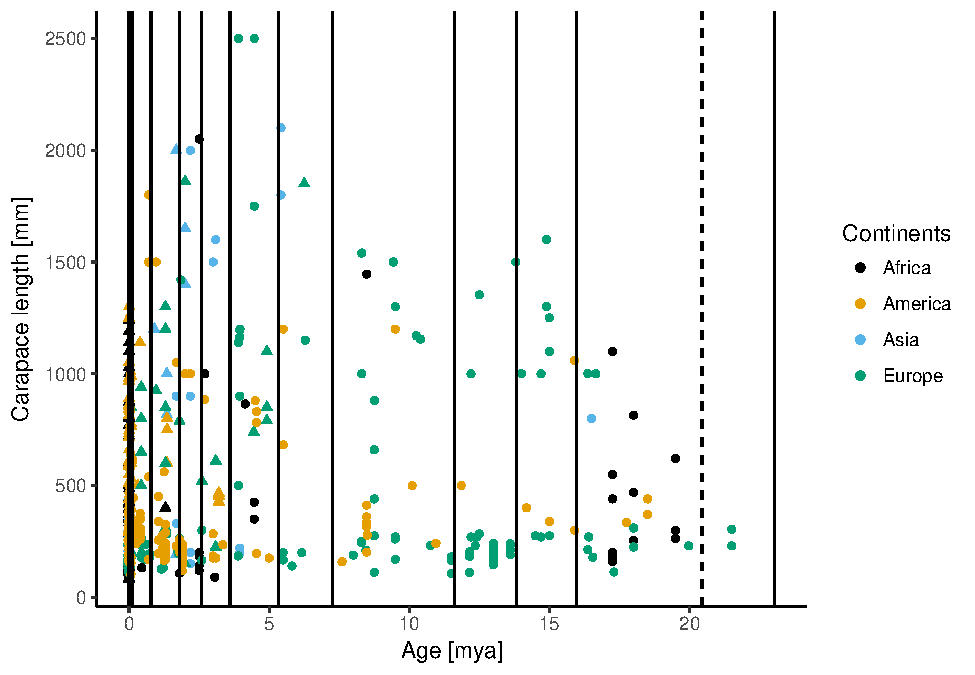
\includegraphics{MA_JJ_files/figure-latex/overviewData-1.pdf}
\caption{Scatterplot of carapace length over time, indicating insular
(triangle) and continental (circles) and colour indicating continents.
Lines indicate stratigraphic stages which were used as time bins, the
dashed line is the border between the two stages of the Lower Miocene,
which were consideres as one time bin.}
\end{figure}

\newpage

\section{Maps}\label{maps}

\subsection{fossil occurences of
testudinidae}\label{fossil-occurences-of-testudinidae}

\begin{figure}[htbp]
\centering
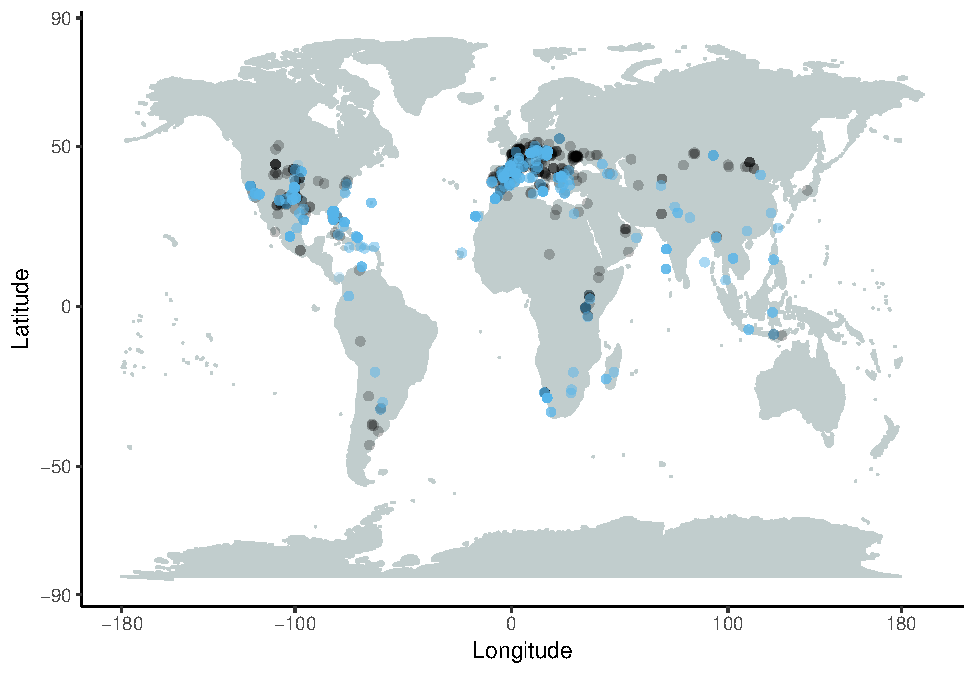
\includegraphics{MA_JJ_files/figure-latex/MapFossilOccurrences-1.pdf}
\caption{Map displaying all fossil occurrences of testudinids, with
color indicating whether relevant literature was available (black if
not) and if it was, whether body size data was available or not (yes and
no, respectively).}
\end{figure}

\newpage

\subsection{body size of testudinidae}\label{body-size-of-testudinidae}

\begin{figure}[htbp]
\centering
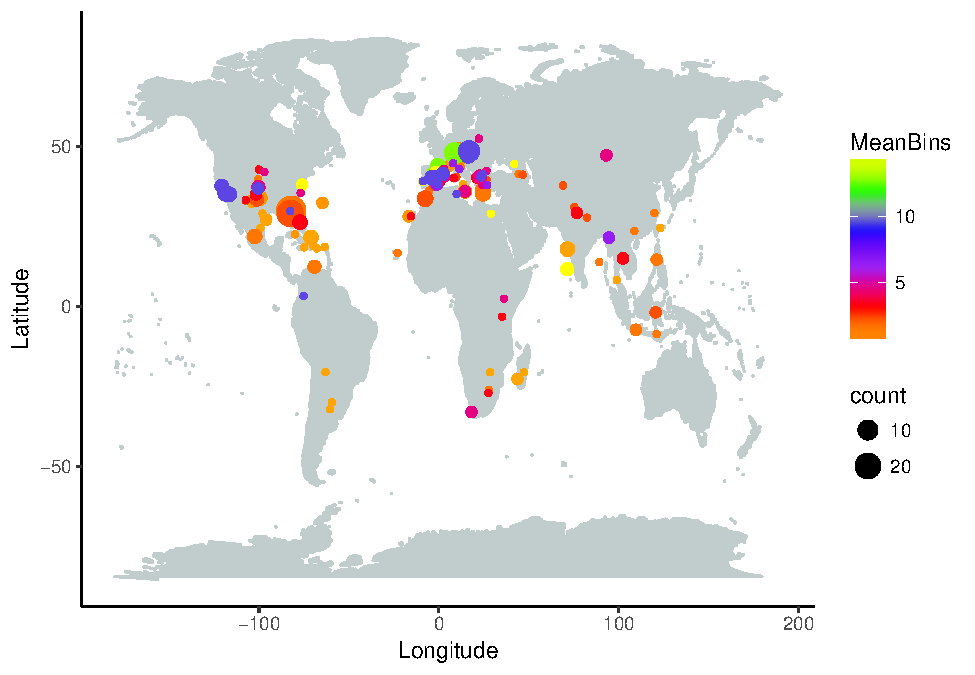
\includegraphics{MA_JJ_files/figure-latex/MapCL-1.pdf}
\caption{Map displaying all localities for which body size data for
testudinids was available in the literature. Size of points denotes
sample size, color denotes approximate age.}
\end{figure}

\begin{longtable}[]{@{}llrr@{}}
\caption{Overview over fossil species per time bin, with sample size and
mean CL.}\tabularnewline
\toprule
EpochBins & Taxon & n & meanCL\tabularnewline
\midrule
\endfirsthead
\toprule
EpochBins & Taxon & n & meanCL\tabularnewline
\midrule
\endhead
Upper Pleistocene & Centrochelys robusta & 1 & 850.0000\tabularnewline
Upper Pleistocene & Chelonoidis denticulata & 1 &
616.0000\tabularnewline
Upper Pleistocene & Chelonoidis lutzae & 1 & 830.0000\tabularnewline
Upper Pleistocene & Chelonoidis marcanoi & 4 & 672.2500\tabularnewline
Upper Pleistocene & Chelonoidis monensis & 1 & 500.0000\tabularnewline
Upper Pleistocene & Chelonoidis sombrerensis & 1 &
990.0000\tabularnewline
Upper Pleistocene & Chelonoidis sp. & 3 & 666.6667\tabularnewline
Upper Pleistocene & Eurotestudo hermanni & 1 & 187.0000\tabularnewline
Upper Pleistocene & gen. indet. & 1 & 813.0000\tabularnewline
Upper Pleistocene & Geochelone sp. & 2 & 475.0000\tabularnewline
Upper Pleistocene & Gopherus agassizi & 1 & 252.0000\tabularnewline
Upper Pleistocene & Gopherus polyphemus & 20 & 292.9700\tabularnewline
Upper Pleistocene & Gopherus praecedens & 1 & 360.0000\tabularnewline
Upper Pleistocene & Hesperotestudo crassiscutata & 6 &
435.1667\tabularnewline
Upper Pleistocene & Hesperotestudo incisa & 1 & 232.7600\tabularnewline
Upper Pleistocene & Hesperotestudo sp. & 2 & 806.5000\tabularnewline
Upper Pleistocene & Hesperotestudo wilsoni & 1 & 226.0000\tabularnewline
Upper Pleistocene & Indotestudo elongata & 1 & 270.0000\tabularnewline
Middle Pleistocene & Centrochelys burchardi & 4 &
722.5000\tabularnewline
Middle Pleistocene & Chelonoidis cubensis & 1 & 1139.0000\tabularnewline
Middle Pleistocene & Eurotestudo aff. hermanni & 2 &
187.0000\tabularnewline
Middle Pleistocene & Eurotestudo hermanni & 2 & 204.0500\tabularnewline
Middle Pleistocene & Geochelone sp. & 1 & 170.0000\tabularnewline
Middle Pleistocene & Gopherus agassizi & 1 & 445.0000\tabularnewline
Middle Pleistocene & Gopherus laticaudatus & 1 & 375.0000\tabularnewline
Middle Pleistocene & Gopherus polyphemus & 31 & 300.4316\tabularnewline
Middle Pleistocene & Hesperotestudo bermudae & 2 &
385.0000\tabularnewline
Middle Pleistocene & Hesperotestudo equicomes & 1 &
340.0000\tabularnewline
Middle Pleistocene & Hesperotestudo sp. & 2 & 1650.0000\tabularnewline
Middle Pleistocene & Testudo kenitrensis & 1 & 132.0000\tabularnewline
Middle Pleistocene & Testudo lunellensis & 4 & 215.4250\tabularnewline
Lower Pleistocene & Centrochelys atlantica & 1 & 400.0000\tabularnewline
Lower Pleistocene & Centrochelys robusta & 3 & 883.3333\tabularnewline
Lower Pleistocene & Cheirogaster cf.~gymnesica & 1 &
789.0000\tabularnewline
Lower Pleistocene & Cheirogaster sp. & 1 & 925.0000\tabularnewline
Lower Pleistocene & Chelonoidis sp. & 3 & 716.6667\tabularnewline
Lower Pleistocene & Eurotestudo globosa & 1 & 263.0000\tabularnewline
Lower Pleistocene & Eurotestudo hermanni & 2 & 205.0000\tabularnewline
Lower Pleistocene & gen. indet. & 1 & 900.0000\tabularnewline
Lower Pleistocene & Geochelone sp. & 1 & 340.0000\tabularnewline
Lower Pleistocene & Gopherus berlandieri & 2 & 225.6500\tabularnewline
Lower Pleistocene & Gopherus flavomarginatus & 1 &
450.0000\tabularnewline
Lower Pleistocene & Gopherus pertenuis & 1 & 1050.0000\tabularnewline
Lower Pleistocene & Gopherus polyphemus & 3 & 254.4667\tabularnewline
Lower Pleistocene & Gopherus sp. & 6 & 233.9667\tabularnewline
Lower Pleistocene & Hesperotestudo crassiscutata & 5 &
285.6000\tabularnewline
Lower Pleistocene & Hesperotestudo incisa & 7 & 234.6286\tabularnewline
Lower Pleistocene & Hesperotestudo mlynarskii & 2 &
184.2500\tabularnewline
Lower Pleistocene & Hesperotestudo sp. & 1 & 1500.0000\tabularnewline
Lower Pleistocene & Hesperotestudo turgida & 1 & 230.0000\tabularnewline
Lower Pleistocene & Megalochelys sondaari & 2 & 909.0000\tabularnewline
Lower Pleistocene & Megalochelys sp. & 3 & 1130.4667\tabularnewline
Lower Pleistocene & Psammobates antiquorum & 1 & 107.8000\tabularnewline
Lower Pleistocene & Testudo changshanesis & 1 & 330.0000\tabularnewline
Lower Pleistocene & Testudo graeca & 1 & 195.0000\tabularnewline
Lower Pleistocene & Testudo hermanni & 2 & 176.5500\tabularnewline
Lower Pleistocene & Testudo marginata & 3 & 270.0000\tabularnewline
Lower Pleistocene & Titanochelon gymnesica & 1 &
1300.0000\tabularnewline
Gelasian & Centrochelys marocana & 1 & 2050.0000\tabularnewline
Gelasian & Eurotestudo cf.~hermanni & 1 & 150.0000\tabularnewline
Gelasian & Gopherus sp. & 15 & 185.7467\tabularnewline
Gelasian & Hesperotestudo campester & 1 & 1000.0000\tabularnewline
Gelasian & Hesperotestudo sp. & 1 & 1000.0000\tabularnewline
Gelasian & Manouria punjabiensis & 1 & 900.0000\tabularnewline
Gelasian & Megalochelys atlas & 3 & 1683.3333\tabularnewline
Gelasian & Testudo aff. kenitrensis & 1 & 142.0000\tabularnewline
Gelasian & Testudo oughlamensis & 1 & 120.0000\tabularnewline
Gelasian & Testudo ranovi & 1 & 200.0000\tabularnewline
Gelasian & Testudo sp. & 2 & 192.0000\tabularnewline
Gelasian & Testudo transcaucasia & 1 & 150.0000\tabularnewline
Gelasian & Titanochelon aff. schafferi & 1 & 1860.0000\tabularnewline
Gelasian & Titanochelon sp. & 1 & 1420.0000\tabularnewline
Piacencian & ``Aldabrachelys'' laetoliensis & 1 &
1000.0000\tabularnewline
Piacencian & Aldabrachelys ? sp. & 2 & 1500.0000\tabularnewline
Piacencian & Centrochelys vulcanica & 1 & 610.0000\tabularnewline
Piacencian & Chelonoidis alburyorum & 4 & 442.7500\tabularnewline
Piacencian & Gopherus canyonensis & 1 & 885.5000\tabularnewline
Piacencian & Hesperotestudo johnstoni & 1 & 235.0000\tabularnewline
Piacencian & Hesperotestudo oelrichi & 1 & 283.8000\tabularnewline
Piacencian & Hesperotestudo riggsi & 2 & 180.5000\tabularnewline
Piacencian & Hesperotestudo sp. & 1 & 176.0000\tabularnewline
Piacencian & Homopus fenestratus & 1 & 90.0000\tabularnewline
Piacencian & Megalochelys atlas & 2 & 1600.0000\tabularnewline
Piacencian & Testudo brevitesta & 2 & 232.5000\tabularnewline
Piacencian & Testudo pecorinii & 1 & 225.0000\tabularnewline
Piacencian & Titanochelon sp. & 1 & 520.0000\tabularnewline
Zanclean & Caudochelys rexroadensis & 2 & 805.5000\tabularnewline
Zanclean & Centrochelys robusta & 3 & 913.3333\tabularnewline
Zanclean & Cheirogaster gymnesica & 1 & 739.0000\tabularnewline
Zanclean & Ergilemys oskarkuhni & 2 & 209.0000\tabularnewline
Zanclean & Geochelone crassa & 1 & 865.0000\tabularnewline
Zanclean & Geochelone s. l. & 1 & 1750.0000\tabularnewline
Zanclean & Geochelone sp. & 2 & 528.0000\tabularnewline
Zanclean & Geochelone stromeri & 2 & 387.5000\tabularnewline
Zanclean & Hesperotestudo riggsi & 1 & 195.8000\tabularnewline
Zanclean & Testudo cf.~graeca & 1 & 185.0000\tabularnewline
Zanclean & Testudo sp. & 4 & 1675.0000\tabularnewline
Zanclean & Titanochelon bacharidisi & 4 & 1040.0000\tabularnewline
Zanclean & Titanochelon perpiniana & 1 & 1140.0000\tabularnewline
Zanclean & Titanochelon schafferi & 1 & 2500.0000\tabularnewline
Messinian & Hesperotestudo orthopygia & 2 & 941.0000\tabularnewline
Messinian & Megalochelys atlas & 2 & 1950.0000\tabularnewline
Messinian & Testudo amiatae & 1 & 140.0000\tabularnewline
Messinian & Testudo graeca & 2 & 183.5000\tabularnewline
Messinian & Testudo sp. & 1 & 200.0000\tabularnewline
Messinian & Titanochelon bolivari & 1 & 1150.0000\tabularnewline
Messinian & Titanochelon schafferi & 1 & 1850.0000\tabularnewline
Tortonian & ``Hadrianus sp.'' & 1 & 1000.0000\tabularnewline
Tortonian & Cheirogaster richardi & 1 & 1155.0000\tabularnewline
Tortonian & Cheirogaster sp. & 2 & 1355.0000\tabularnewline
Tortonian & gen. indet. & 3 & 660.0000\tabularnewline
Tortonian & Geochelone hesterna & 1 & 278.0000\tabularnewline
Tortonian & Geochelone sp. & 2 & 973.0000\tabularnewline
Tortonian & Gopherus ? sp. & 1 & 500.0000\tabularnewline
Tortonian & Gopherus mohavetus & 5 & 324.8000\tabularnewline
Tortonian & Hesperotestudo alleni & 1 & 240.9000\tabularnewline
Tortonian & Hesperotestudo riggsi & 2 & 159.5000\tabularnewline
Tortonian & Hesperotestudo sp. & 1 & 1200.0000\tabularnewline
Tortonian & Paleotestudo sp. & 3 & 233.6667\tabularnewline
Tortonian & Testudo burgenlandica & 2 & 193.5000\tabularnewline
Tortonian & Testudo catalaunica & 4 & 157.0000\tabularnewline
Tortonian & Testudo cf.~promarginata & 5 & 250.0000\tabularnewline
Tortonian & Testudo graeca & 1 & 210.0000\tabularnewline
Tortonian & Testudo s. s. & 1 & 189.0000\tabularnewline
Tortonian & Testudo sp. & 7 & 243.1571\tabularnewline
Tortonian & Titanochelon bolivari & 1 & 1300.0000\tabularnewline
Tortonian & Titanochelon cf.~bolivari & 1 & 1500.0000\tabularnewline
Serravallian & Cheirogaster sp. & 2 & 1250.0000\tabularnewline
Serravallian & gen. indet. & 1 & 270.0000\tabularnewline
Serravallian & Gopherus ? sp. & 1 & 500.0000\tabularnewline
Serravallian & Paleotestudo antiqua & 18 & 203.0556\tabularnewline
Serravallian & Paleotestudo cf.~sp. & 1 & 270.0000\tabularnewline
Serravallian & Testudo catalaunica & 1 & 232.0000\tabularnewline
Serravallian & Testudo steinheimensis & 2 & 169.3500\tabularnewline
Serravallian & Titanochelon bolivari & 1 & 1353.0000\tabularnewline
Langhian & Caudochelys ducateli & 1 & 339.9000\tabularnewline
Langhian & Chelonoidis sp. & 3 & 553.3333\tabularnewline
Langhian & Ergilemys sp. & 1 & 1000.0000\tabularnewline
Langhian & gen. indet. & 1 & 1000.0000\tabularnewline
Langhian & Paleotestudo antiqua & 1 & 275.0000\tabularnewline
Langhian & Paleotestudo cf.~sp. & 1 & 270.0000\tabularnewline
Langhian & Testudo kalksburgensis & 1 & 275.0000\tabularnewline
Langhian & Testudo sp. & 1 & 400.0000\tabularnewline
Langhian & Titanochelon bolivari & 2 & 1175.0000\tabularnewline
Langhian & Titanochelon cf.~bolivari & 2 & 1450.0000\tabularnewline
Burdigalian/Aquitanian & Caudochelys williamsi & 1 &
334.0000\tabularnewline
Burdigalian/Aquitanian & gen. indet. & 1 & 270.0000\tabularnewline
Burdigalian/Aquitanian & Geochelone sp. & 2 & 900.0000\tabularnewline
Burdigalian/Aquitanian & Geochelone tedwhitei & 2 &
405.0000\tabularnewline
Burdigalian/Aquitanian & Impregnochelys pachytectis & 1 &
620.0000\tabularnewline
Burdigalian/Aquitanian & Mesocherus orangeus & 5 &
180.0000\tabularnewline
Burdigalian/Aquitanian & Namibchersus aff. namaquensis & 3 &
696.6667\tabularnewline
Burdigalian/Aquitanian & Namibchersus namaquensis & 6 &
428.8333\tabularnewline
Burdigalian/Aquitanian & Paleotestudo cf.~antiqua & 1 &
113.0000\tabularnewline
Burdigalian/Aquitanian & Paleotestudo sp. & 1 & 179.3000\tabularnewline
Burdigalian/Aquitanian & Testudo kalksburgensis & 2 &
227.5000\tabularnewline
Burdigalian/Aquitanian & Testudo promarginata & 3 &
281.5667\tabularnewline
Burdigalian/Aquitanian & Testudo rectogularis & 1 &
213.0000\tabularnewline
Burdigalian/Aquitanian & Titanochelon cf.~perpiniana & 1 &
1001.0000\tabularnewline
\bottomrule
\end{longtable}

\begin{longtable}[]{@{}lrr@{}}
\caption{General overview over fossil species, with sample size and mean
CL}\tabularnewline
\toprule
Taxon & n & meanCL\tabularnewline
\midrule
\endfirsthead
\toprule
Taxon & n & meanCL\tabularnewline
\midrule
\endhead
``Aldabrachelys'' laetoliensis & 1 & 1000.0000\tabularnewline
``Hadrianus sp.'' & 1 & 1000.0000\tabularnewline
Aldabrachelys ? sp. & 2 & 1500.0000\tabularnewline
Caudochelys ducateli & 1 & 339.9000\tabularnewline
Caudochelys rexroadensis & 2 & 805.5000\tabularnewline
Caudochelys williamsi & 1 & 334.0000\tabularnewline
Centrochelys atlantica & 1 & 400.0000\tabularnewline
Centrochelys burchardi & 4 & 722.5000\tabularnewline
Centrochelys marocana & 1 & 2050.0000\tabularnewline
Centrochelys robusta & 7 & 891.4286\tabularnewline
Centrochelys vulcanica & 1 & 610.0000\tabularnewline
Cheirogaster cf.~gymnesica & 1 & 789.0000\tabularnewline
Cheirogaster gymnesica & 1 & 739.0000\tabularnewline
Cheirogaster richardi & 1 & 1155.0000\tabularnewline
Cheirogaster sp. & 5 & 1227.0000\tabularnewline
Chelonoidis alburyorum & 4 & 442.7500\tabularnewline
Chelonoidis cubensis & 1 & 1139.0000\tabularnewline
Chelonoidis denticulata & 1 & 616.0000\tabularnewline
Chelonoidis lutzae & 1 & 830.0000\tabularnewline
Chelonoidis marcanoi & 4 & 672.2500\tabularnewline
Chelonoidis monensis & 1 & 500.0000\tabularnewline
Chelonoidis sombrerensis & 1 & 990.0000\tabularnewline
Chelonoidis sp. & 9 & 645.5556\tabularnewline
Ergilemys oskarkuhni & 2 & 209.0000\tabularnewline
Ergilemys sp. & 1 & 1000.0000\tabularnewline
Eurotestudo aff. hermanni & 2 & 187.0000\tabularnewline
Eurotestudo cf.~hermanni & 1 & 150.0000\tabularnewline
Eurotestudo globosa & 1 & 263.0000\tabularnewline
Eurotestudo hermanni & 5 & 201.0200\tabularnewline
gen. indet. & 8 & 654.1250\tabularnewline
Geochelone crassa & 1 & 865.0000\tabularnewline
Geochelone hesterna & 1 & 278.0000\tabularnewline
Geochelone s. l. & 1 & 1750.0000\tabularnewline
Geochelone sp. & 10 & 626.2000\tabularnewline
Geochelone stromeri & 2 & 387.5000\tabularnewline
Geochelone tedwhitei & 2 & 405.0000\tabularnewline
Gopherus ? sp. & 2 & 500.0000\tabularnewline
Gopherus agassizi & 2 & 348.5000\tabularnewline
Gopherus berlandieri & 2 & 225.6500\tabularnewline
Gopherus canyonensis & 1 & 885.5000\tabularnewline
Gopherus flavomarginatus & 1 & 450.0000\tabularnewline
Gopherus laticaudatus & 1 & 375.0000\tabularnewline
Gopherus mohavetus & 5 & 324.8000\tabularnewline
Gopherus pertenuis & 1 & 1050.0000\tabularnewline
Gopherus polyphemus & 54 & 295.1144\tabularnewline
Gopherus praecedens & 1 & 360.0000\tabularnewline
Gopherus sp. & 21 & 199.5238\tabularnewline
Hesperotestudo alleni & 1 & 240.9000\tabularnewline
Hesperotestudo bermudae & 2 & 385.0000\tabularnewline
Hesperotestudo campester & 1 & 1000.0000\tabularnewline
Hesperotestudo crassiscutata & 11 & 367.1818\tabularnewline
Hesperotestudo equicomes & 1 & 340.0000\tabularnewline
Hesperotestudo incisa & 8 & 234.3950\tabularnewline
Hesperotestudo johnstoni & 1 & 235.0000\tabularnewline
Hesperotestudo mlynarskii & 2 & 184.2500\tabularnewline
Hesperotestudo oelrichi & 1 & 283.8000\tabularnewline
Hesperotestudo orthopygia & 2 & 941.0000\tabularnewline
Hesperotestudo riggsi & 5 & 175.1600\tabularnewline
Hesperotestudo sp. & 8 & 1098.6250\tabularnewline
Hesperotestudo turgida & 1 & 230.0000\tabularnewline
Hesperotestudo wilsoni & 1 & 226.0000\tabularnewline
Homopus fenestratus & 1 & 90.0000\tabularnewline
Impregnochelys pachytectis & 1 & 620.0000\tabularnewline
Indotestudo elongata & 1 & 270.0000\tabularnewline
Manouria punjabiensis & 1 & 900.0000\tabularnewline
Megalochelys atlas & 7 & 1735.7143\tabularnewline
Megalochelys sondaari & 2 & 909.0000\tabularnewline
Megalochelys sp. & 3 & 1130.4667\tabularnewline
Mesocherus orangeus & 5 & 180.0000\tabularnewline
Namibchersus aff. namaquensis & 3 & 696.6667\tabularnewline
Namibchersus namaquensis & 6 & 428.8333\tabularnewline
Paleotestudo antiqua & 19 & 206.8421\tabularnewline
Paleotestudo cf.~antiqua & 1 & 113.0000\tabularnewline
Paleotestudo cf.~sp. & 2 & 270.0000\tabularnewline
Paleotestudo sp. & 4 & 220.0750\tabularnewline
Psammobates antiquorum & 1 & 107.8000\tabularnewline
Testudo aff. kenitrensis & 1 & 142.0000\tabularnewline
Testudo amiatae & 1 & 140.0000\tabularnewline
Testudo brevitesta & 2 & 232.5000\tabularnewline
Testudo burgenlandica & 2 & 193.5000\tabularnewline
Testudo catalaunica & 5 & 172.0000\tabularnewline
Testudo cf.~graeca & 1 & 185.0000\tabularnewline
Testudo cf.~promarginata & 5 & 250.0000\tabularnewline
Testudo changshanesis & 1 & 330.0000\tabularnewline
Testudo graeca & 4 & 193.0000\tabularnewline
Testudo hermanni & 2 & 176.5500\tabularnewline
Testudo kalksburgensis & 3 & 243.3333\tabularnewline
Testudo kenitrensis & 1 & 132.0000\tabularnewline
Testudo lunellensis & 4 & 215.4250\tabularnewline
Testudo marginata & 3 & 270.0000\tabularnewline
Testudo oughlamensis & 1 & 120.0000\tabularnewline
Testudo pecorinii & 1 & 225.0000\tabularnewline
Testudo promarginata & 3 & 281.5667\tabularnewline
Testudo ranovi & 1 & 200.0000\tabularnewline
Testudo rectogularis & 1 & 213.0000\tabularnewline
Testudo s. s. & 1 & 189.0000\tabularnewline
Testudo sp. & 15 & 625.7400\tabularnewline
Testudo steinheimensis & 2 & 169.3500\tabularnewline
Testudo transcaucasia & 1 & 150.0000\tabularnewline
Titanochelon aff. schafferi & 1 & 1860.0000\tabularnewline
Titanochelon bacharidisi & 4 & 1040.0000\tabularnewline
Titanochelon bolivari & 5 & 1230.6000\tabularnewline
Titanochelon cf.~bolivari & 3 & 1466.6667\tabularnewline
Titanochelon cf.~perpiniana & 1 & 1001.0000\tabularnewline
Titanochelon gymnesica & 1 & 1300.0000\tabularnewline
Titanochelon perpiniana & 1 & 1140.0000\tabularnewline
Titanochelon schafferi & 2 & 2175.0000\tabularnewline
Titanochelon sp. & 2 & 970.0000\tabularnewline
\bottomrule
\end{longtable}

\begin{longtable}[]{@{}llrr@{}}
\caption{Overview over genera (modern and fossil) per time bin, with
sample sizes and mean CL.}\tabularnewline
\toprule
EpochBins & Genus & n & meanCL\tabularnewline
\midrule
\endfirsthead
\toprule
EpochBins & Genus & n & meanCL\tabularnewline
\midrule
\endhead
Modern & Aldabrachelys & 12 & 974.5833\tabularnewline
Modern & Astrochelys & 14 & 366.2143\tabularnewline
Modern & Centrochelys & 3 & 493.3333\tabularnewline
Modern & Chelonoidis & 45 & 531.5178\tabularnewline
Modern & Chersina & 15 & 176.2667\tabularnewline
Modern & Cylindraspis & 5 & 724.0000\tabularnewline
Modern & Geochelone & 8 & 252.1250\tabularnewline
Modern & Gopherus & 23 & 302.4839\tabularnewline
Modern & Hesperotestudo & 1 & 250.0000\tabularnewline
Modern & Homopus & 7 & 139.2857\tabularnewline
Modern & Indotestudo & 16 & 242.9875\tabularnewline
Modern & Kinixys & 15 & 213.0667\tabularnewline
Modern & Malacochersus & 2 & 166.5000\tabularnewline
Modern & Manouria & 9 & 380.7778\tabularnewline
Modern & Psammobates & 17 & 113.4118\tabularnewline
Modern & Pyxis & 16 & 124.1875\tabularnewline
Modern & Stigmochelys & 6 & 405.3333\tabularnewline
Modern & Testudo & 39 & 197.5436\tabularnewline
Upper Pleistocene & Centrochelys & 1 & 850.0000\tabularnewline
Upper Pleistocene & Chelonoidis & 11 & 693.1818\tabularnewline
Upper Pleistocene & Eurotestudo & 1 & 187.0000\tabularnewline
Upper Pleistocene & gen. & 1 & 813.0000\tabularnewline
Upper Pleistocene & Geochelone & 2 & 475.0000\tabularnewline
Upper Pleistocene & Gopherus & 22 & 294.1545\tabularnewline
Upper Pleistocene & Hesperotestudo & 10 & 468.2760\tabularnewline
Upper Pleistocene & Indotestudo & 1 & 270.0000\tabularnewline
Middle Pleistocene & Centrochelys & 4 & 722.5000\tabularnewline
Middle Pleistocene & Chelonoidis & 1 & 1139.0000\tabularnewline
Middle Pleistocene & Eurotestudo & 4 & 195.5250\tabularnewline
Middle Pleistocene & Geochelone & 1 & 170.0000\tabularnewline
Middle Pleistocene & Gopherus & 33 & 307.0721\tabularnewline
Middle Pleistocene & Hesperotestudo & 5 & 882.0000\tabularnewline
Middle Pleistocene & Testudo & 5 & 198.7400\tabularnewline
Lower Pleistocene & Centrochelys & 4 & 762.5000\tabularnewline
Lower Pleistocene & Cheirogaster & 2 & 857.0000\tabularnewline
Lower Pleistocene & Chelonoidis & 3 & 716.6667\tabularnewline
Lower Pleistocene & Eurotestudo & 4 & 201.5250\tabularnewline
Lower Pleistocene & gen. & 1 & 900.0000\tabularnewline
Lower Pleistocene & Geochelone & 1 & 340.0000\tabularnewline
Lower Pleistocene & Gopherus & 13 & 316.8077\tabularnewline
Lower Pleistocene & Hesperotestudo & 16 & 323.0562\tabularnewline
Lower Pleistocene & Megalochelys & 5 & 1041.8800\tabularnewline
Lower Pleistocene & Psammobates & 1 & 107.8000\tabularnewline
Lower Pleistocene & Testudo & 6 & 259.1667\tabularnewline
Lower Pleistocene & Titanochelon & 1 & 1300.0000\tabularnewline
Gelasian & Centrochelys & 1 & 2050.0000\tabularnewline
Gelasian & Eurotestudo & 1 & 150.0000\tabularnewline
Gelasian & Gopherus & 15 & 185.7467\tabularnewline
Gelasian & Hesperotestudo & 2 & 1000.0000\tabularnewline
Gelasian & Manouria & 1 & 900.0000\tabularnewline
Gelasian & Megalochelys & 3 & 1683.3333\tabularnewline
Gelasian & Testudo & 6 & 166.0000\tabularnewline
Gelasian & Titanochelon & 2 & 1640.0000\tabularnewline
Piacencian & Aldabrachelys & 3 & 1333.3333\tabularnewline
Piacencian & Centrochelys & 1 & 610.0000\tabularnewline
Piacencian & Chelonoidis & 4 & 442.7500\tabularnewline
Piacencian & Gopherus & 1 & 885.5000\tabularnewline
Piacencian & Hesperotestudo & 5 & 211.1600\tabularnewline
Piacencian & Homopus & 1 & 90.0000\tabularnewline
Piacencian & Megalochelys & 2 & 1600.0000\tabularnewline
Piacencian & Testudo & 3 & 230.0000\tabularnewline
Piacencian & Titanochelon & 1 & 520.0000\tabularnewline
Zanclean & Caudochelys & 2 & 805.5000\tabularnewline
Zanclean & Centrochelys & 3 & 913.3333\tabularnewline
Zanclean & Cheirogaster & 1 & 739.0000\tabularnewline
Zanclean & Ergilemys & 2 & 209.0000\tabularnewline
Zanclean & Geochelone & 6 & 741.0000\tabularnewline
Zanclean & Hesperotestudo & 1 & 195.8000\tabularnewline
Zanclean & Testudo & 5 & 1377.0000\tabularnewline
Zanclean & Titanochelon & 6 & 1300.0000\tabularnewline
Messinian & Hesperotestudo & 2 & 941.0000\tabularnewline
Messinian & Megalochelys & 2 & 1950.0000\tabularnewline
Messinian & Testudo & 4 & 176.7500\tabularnewline
Messinian & Titanochelon & 2 & 1500.0000\tabularnewline
Tortonian & ``Hadrianus'' & 1 & 1000.0000\tabularnewline
Tortonian & Cheirogaster & 3 & 1288.3333\tabularnewline
Tortonian & gen. & 3 & 660.0000\tabularnewline
Tortonian & Geochelone & 3 & 741.3333\tabularnewline
Tortonian & Gopherus & 6 & 354.0000\tabularnewline
Tortonian & Hesperotestudo & 4 & 439.9750\tabularnewline
Tortonian & Paleotestudo & 3 & 233.6667\tabularnewline
Tortonian & Testudo & 20 & 218.3050\tabularnewline
Tortonian & Titanochelon & 2 & 1400.0000\tabularnewline
Serravallian & Cheirogaster & 2 & 1250.0000\tabularnewline
Serravallian & gen. & 1 & 270.0000\tabularnewline
Serravallian & Gopherus & 1 & 500.0000\tabularnewline
Serravallian & Paleotestudo & 19 & 206.5789\tabularnewline
Serravallian & Testudo & 3 & 190.2333\tabularnewline
Serravallian & Titanochelon & 1 & 1353.0000\tabularnewline
Langhian & Caudochelys & 1 & 339.9000\tabularnewline
Langhian & Chelonoidis & 3 & 553.3333\tabularnewline
Langhian & Ergilemys & 1 & 1000.0000\tabularnewline
Langhian & gen. & 1 & 1000.0000\tabularnewline
Langhian & Paleotestudo & 2 & 272.5000\tabularnewline
Langhian & Testudo & 2 & 337.5000\tabularnewline
Langhian & Titanochelon & 4 & 1312.5000\tabularnewline
Burdigalian/Aquitanian & Caudochelys & 1 & 334.0000\tabularnewline
Burdigalian/Aquitanian & gen. & 1 & 270.0000\tabularnewline
Burdigalian/Aquitanian & Geochelone & 4 & 652.5000\tabularnewline
Burdigalian/Aquitanian & Impregnochelys & 1 & 620.0000\tabularnewline
Burdigalian/Aquitanian & Mesocherus & 5 & 180.0000\tabularnewline
Burdigalian/Aquitanian & Namibchersus & 9 & 518.1111\tabularnewline
Burdigalian/Aquitanian & Paleotestudo & 2 & 146.1500\tabularnewline
Burdigalian/Aquitanian & Testudo & 6 & 252.1167\tabularnewline
Burdigalian/Aquitanian & Titanochelon & 1 & 1001.0000\tabularnewline
\bottomrule
\end{longtable}

\begin{longtable}[]{@{}lrr@{}}
\caption{General overview over genera, with sample sizes and mean
CL.}\tabularnewline
\toprule
Genus & n & meanCL\tabularnewline
\midrule
\endfirsthead
\toprule
Genus & n & meanCL\tabularnewline
\midrule
\endhead
``Hadrianus'' & 1 & 1000.0000\tabularnewline
Aldabrachelys & 15 & 1046.3333\tabularnewline
Astrochelys & 14 & 366.2143\tabularnewline
Caudochelys & 4 & 571.2250\tabularnewline
Centrochelys & 17 & 804.1176\tabularnewline
Cheirogaster & 8 & 1102.2500\tabularnewline
Chelonoidis & 67 & 571.0940\tabularnewline
Chersina & 15 & 176.2667\tabularnewline
Cylindraspis & 5 & 724.0000\tabularnewline
Ergilemys & 3 & 472.6667\tabularnewline
Eurotestudo & 10 & 192.5200\tabularnewline
gen. & 8 & 654.1250\tabularnewline
Geochelone & 25 & 510.2800\tabularnewline
Gopherus & 114 & 298.0361\tabularnewline
Hesperotestudo & 46 & 465.3296\tabularnewline
Homopus & 8 & 133.1250\tabularnewline
Impregnochelys & 1 & 620.0000\tabularnewline
Indotestudo & 17 & 244.5765\tabularnewline
Kinixys & 15 & 213.0667\tabularnewline
Malacochersus & 2 & 166.5000\tabularnewline
Manouria & 10 & 432.7000\tabularnewline
Megalochelys & 12 & 1446.6167\tabularnewline
Mesocherus & 5 & 180.0000\tabularnewline
Namibchersus & 9 & 518.1111\tabularnewline
Paleotestudo & 26 & 210.1269\tabularnewline
Psammobates & 18 & 113.1000\tabularnewline
Pyxis & 16 & 124.1875\tabularnewline
Stigmochelys & 6 & 405.3333\tabularnewline
Testudo & 99 & 269.2465\tabularnewline
Titanochelon & 20 & 1315.2000\tabularnewline
\bottomrule
\end{longtable}

\newpage

\section{Sampling Accumulation
Curves}\label{sampling-accumulation-curves}

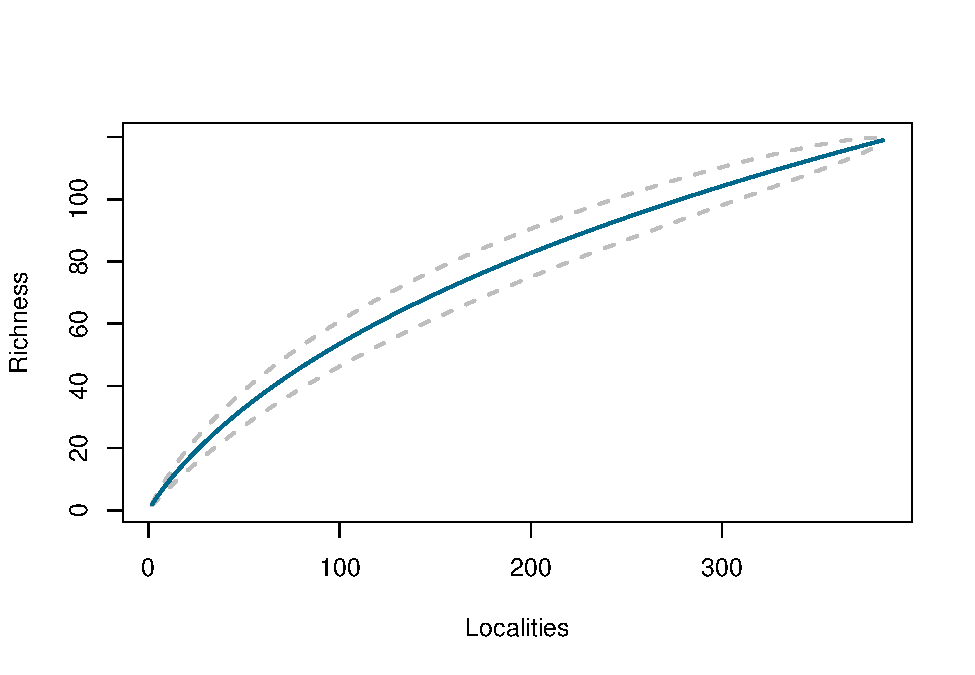
\includegraphics{MA_JJ_files/figure-latex/SACSpecies-1.pdf}
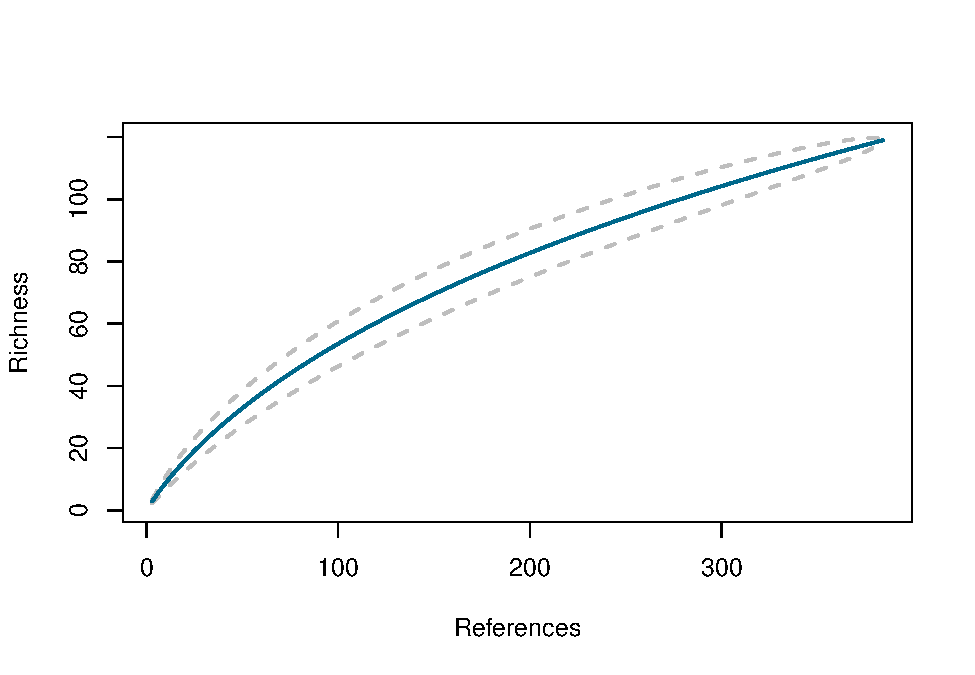
\includegraphics{MA_JJ_files/figure-latex/SACSpecies-2.pdf}

\begin{figure}[htbp]
\centering
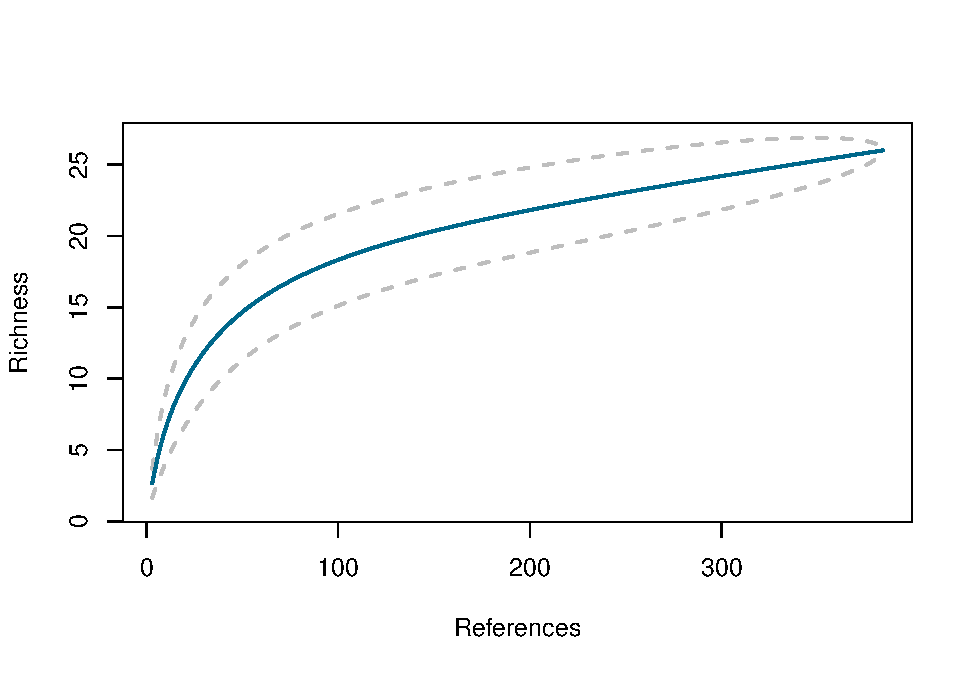
\includegraphics{MA_JJ_files/figure-latex/SACGenera-1.pdf}
\caption{Sampling Accumulation Curve of fossil genera per reference}
\end{figure}

\begin{figure}[htbp]
\centering
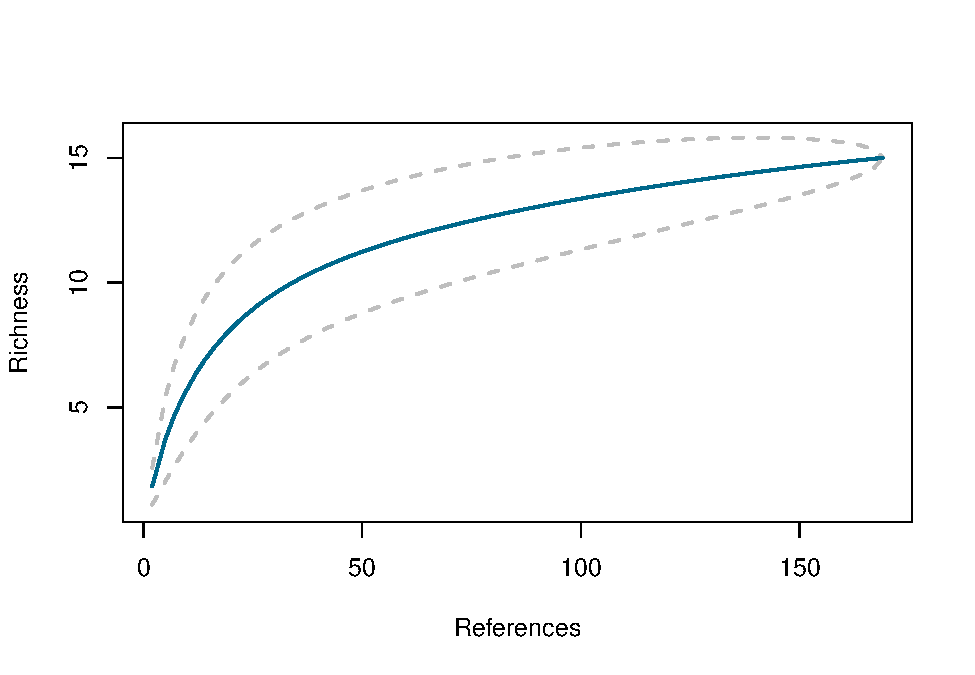
\includegraphics{MA_JJ_files/figure-latex/SACGEurasia-1.pdf}
\caption{Sampling Accumulation Curve of fossil genera per reference,
Eurasia}
\end{figure}

\begin{figure}[htbp]
\centering
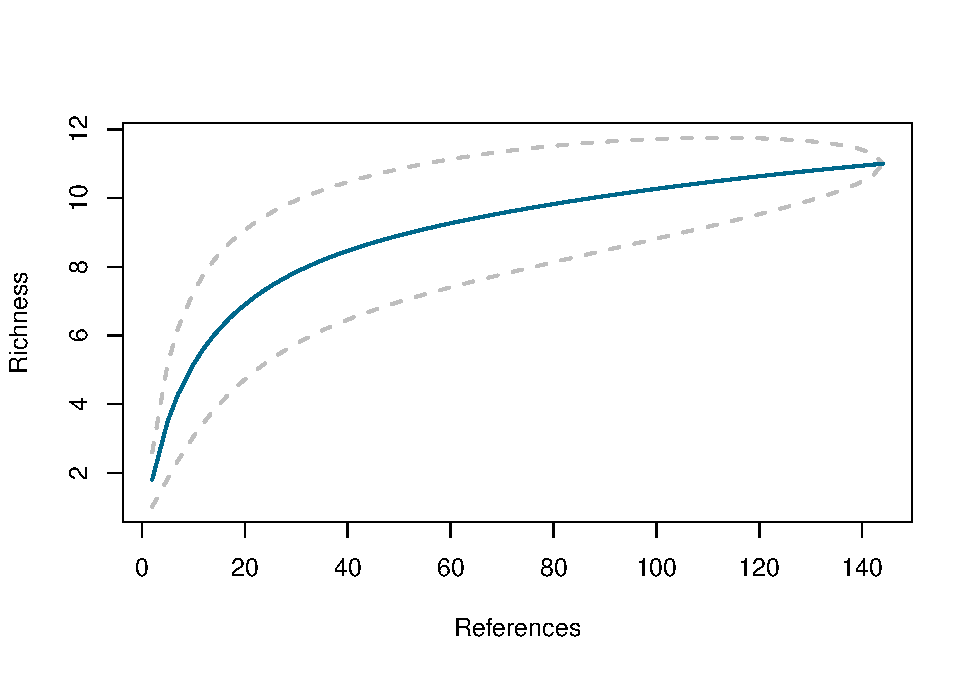
\includegraphics{MA_JJ_files/figure-latex/SACGEurope-1.pdf}
\caption{Sampling Accumulation Curve of fossil genera per reference,
Europe}
\end{figure}

\begin{figure}[htbp]
\centering
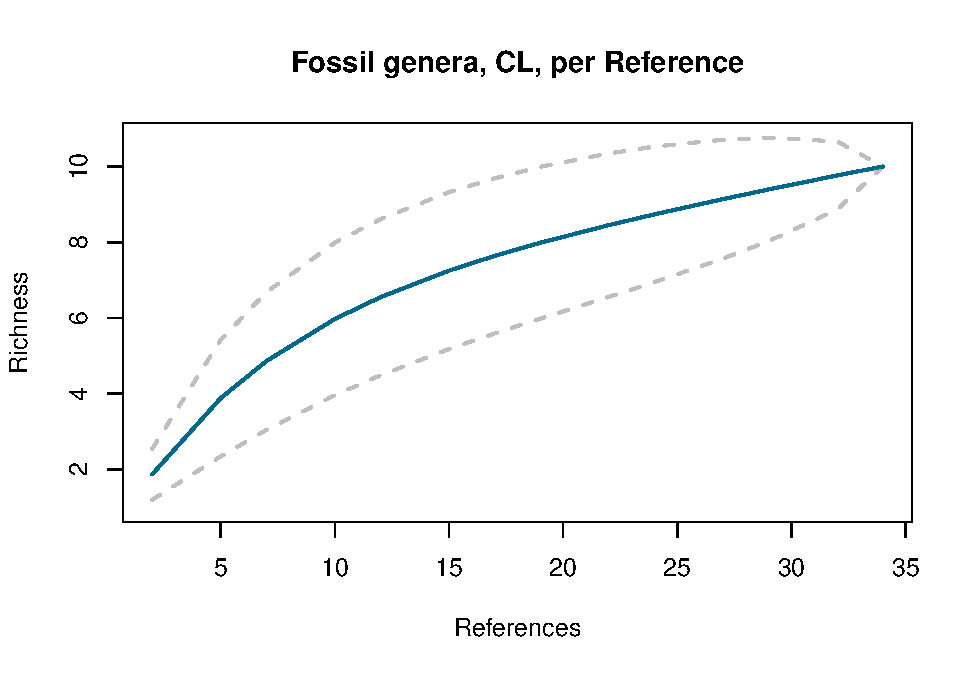
\includegraphics{MA_JJ_files/figure-latex/SACGAfrica-1.pdf}
\caption{Sampling Accumulation Curve of fossil genera per reference,
Africa}
\end{figure}

\begin{figure}[htbp]
\centering
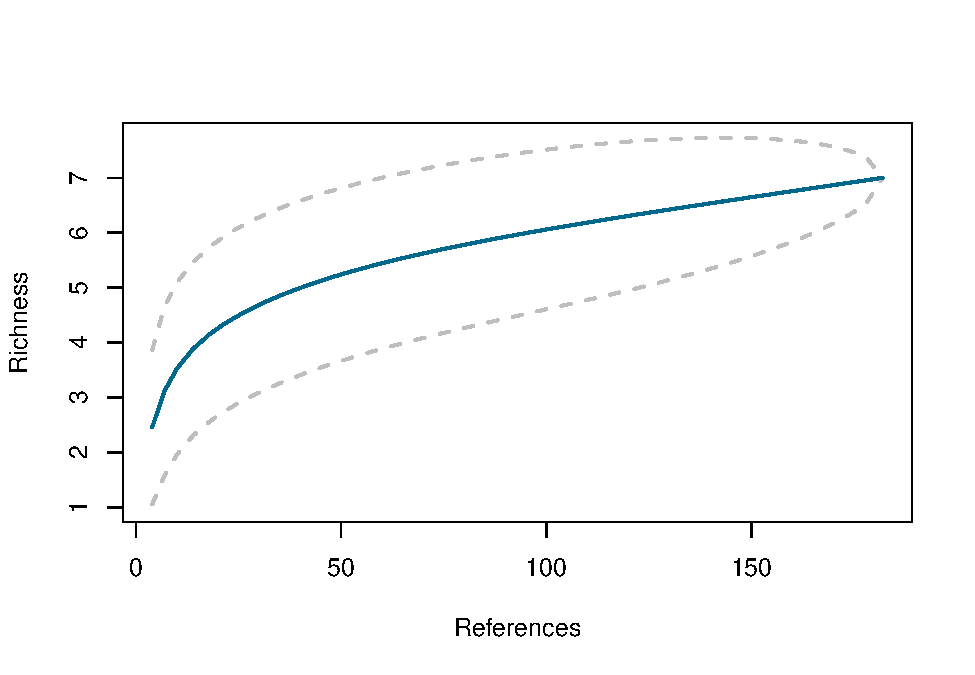
\includegraphics{MA_JJ_files/figure-latex/SACGAmerica-1.pdf}
\caption{Sampling Accumulation Curve of fossil genera per reference,
America}
\end{figure}

\begin{figure}[htbp]
\centering
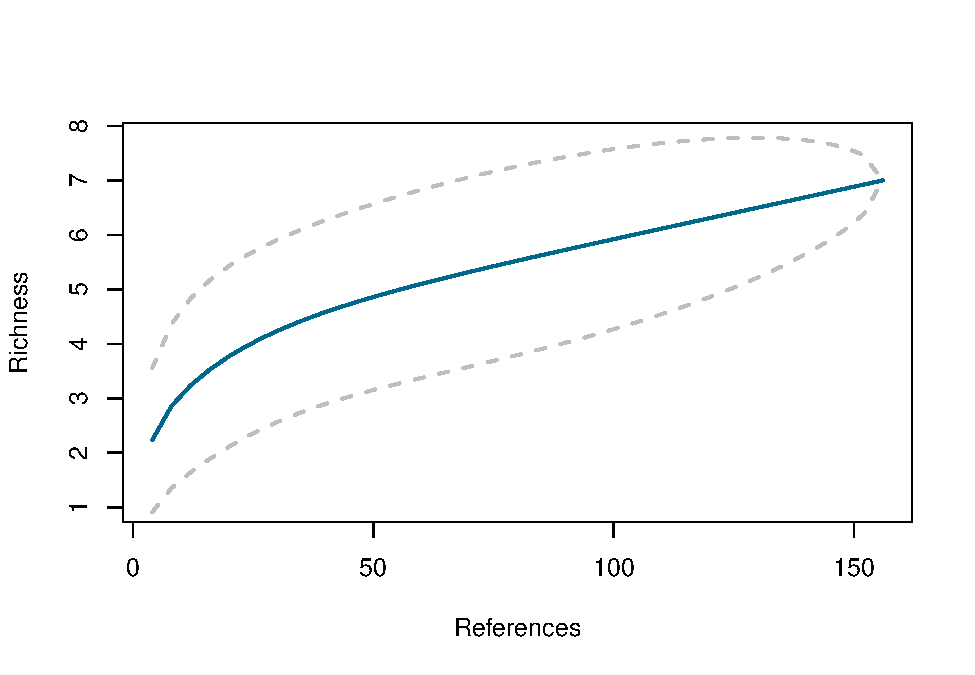
\includegraphics{MA_JJ_files/figure-latex/SACGNAmerica-1.pdf}
\caption{Sampling Accumulation Curve of fossil genera per reference,
N-America}
\end{figure}

\begin{figure}[htbp]
\centering
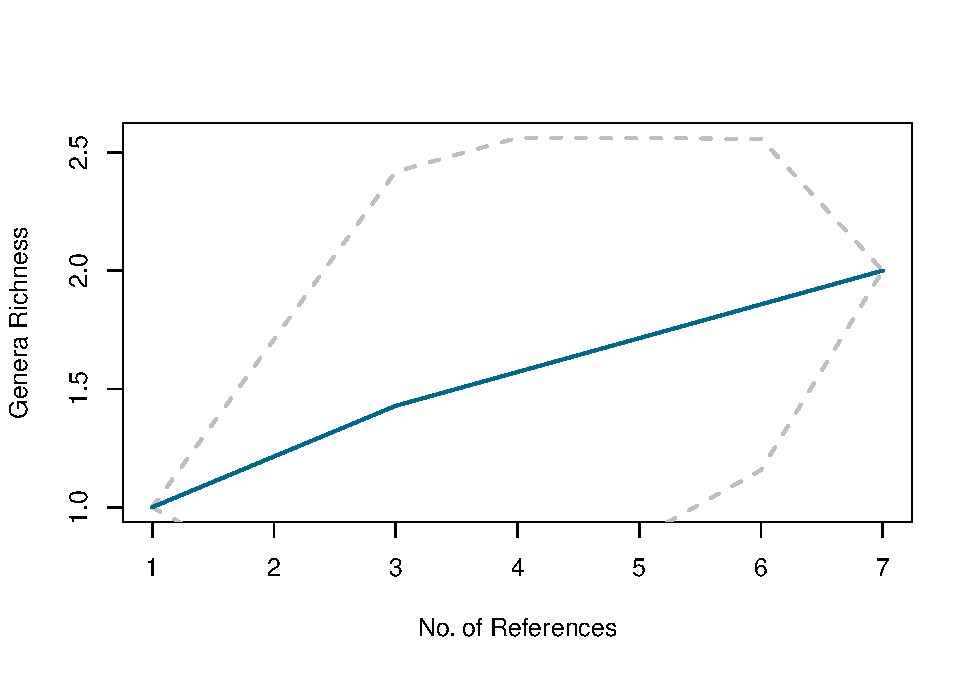
\includegraphics{MA_JJ_files/figure-latex/SACGSAmerica-1.pdf}
\caption{Sampling Accumulation Curve of fossil genera per reference,
S-America}
\end{figure}

\begin{figure}[htbp]
\centering
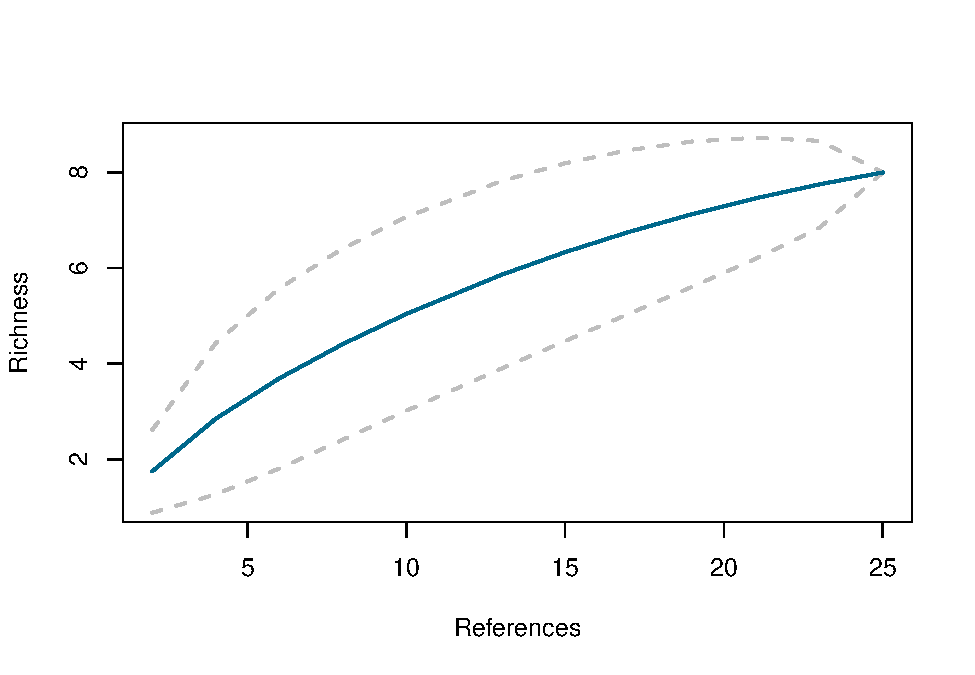
\includegraphics{MA_JJ_files/figure-latex/SACGAsia-1.pdf}
\caption{Sampling Accumulation Curve of fossil genera per reference,
Asia}
\end{figure}

\newpage

\section{Histograms}\label{histograms}

\subsection{all}\label{all}

\begin{verbatim}
## `stat_bin()` using `bins = 30`. Pick better value with `binwidth`.
\end{verbatim}

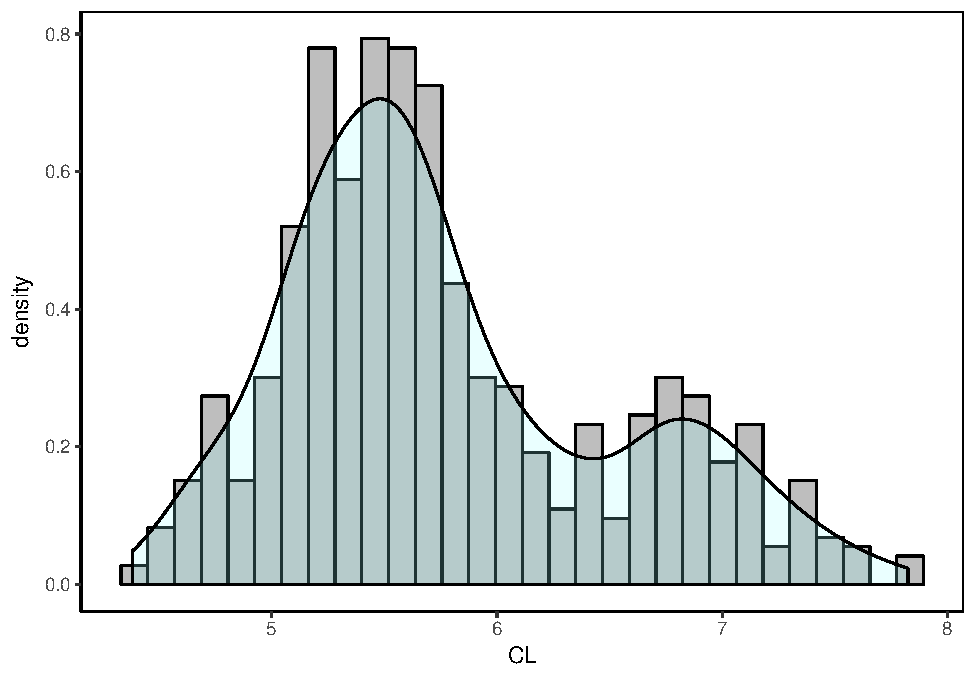
\includegraphics{MA_JJ_files/figure-latex/HistAll-1.pdf}
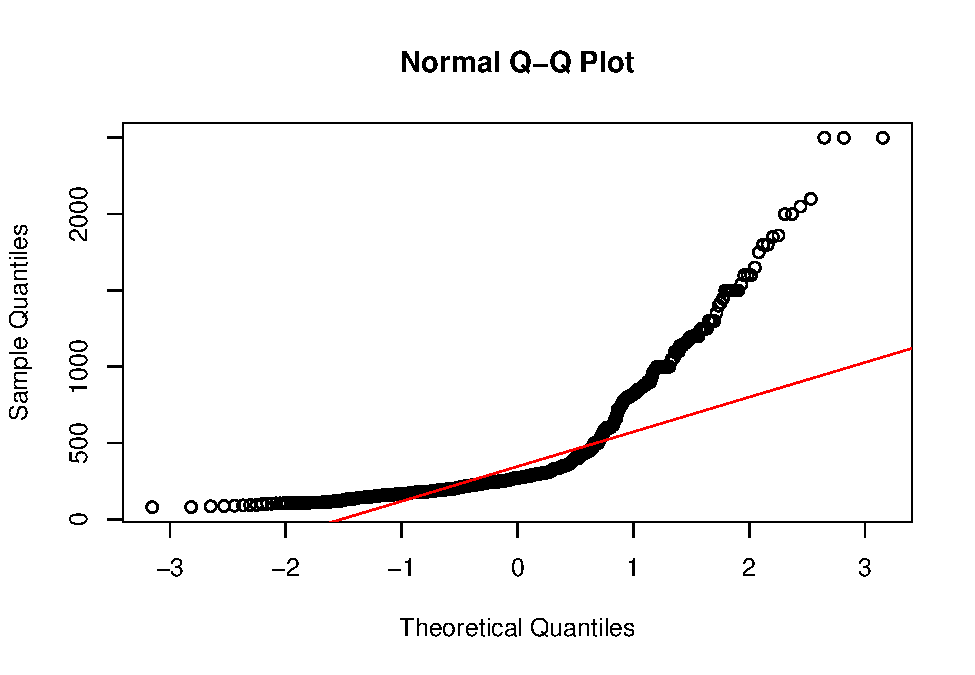
\includegraphics{MA_JJ_files/figure-latex/normalDistribution-1.pdf}
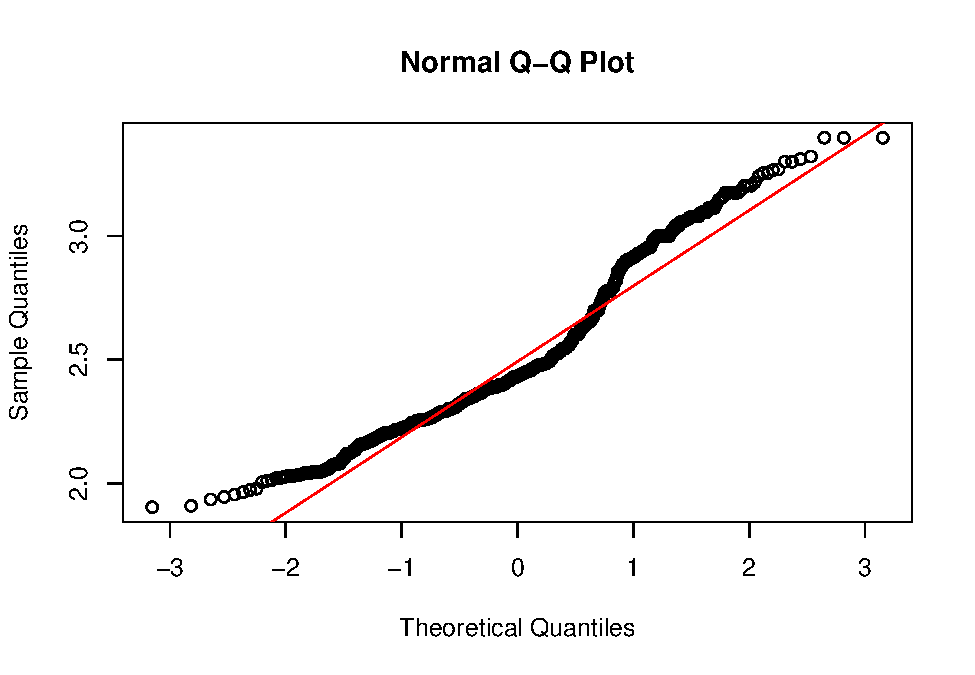
\includegraphics{MA_JJ_files/figure-latex/normalDistribution-2.pdf}

\newpage

\subsection{per time bin}\label{per-time-bin}

\begin{verbatim}
## `stat_bin()` using `bins = 30`. Pick better value with `binwidth`.
\end{verbatim}

\begin{figure}[htbp]
\centering
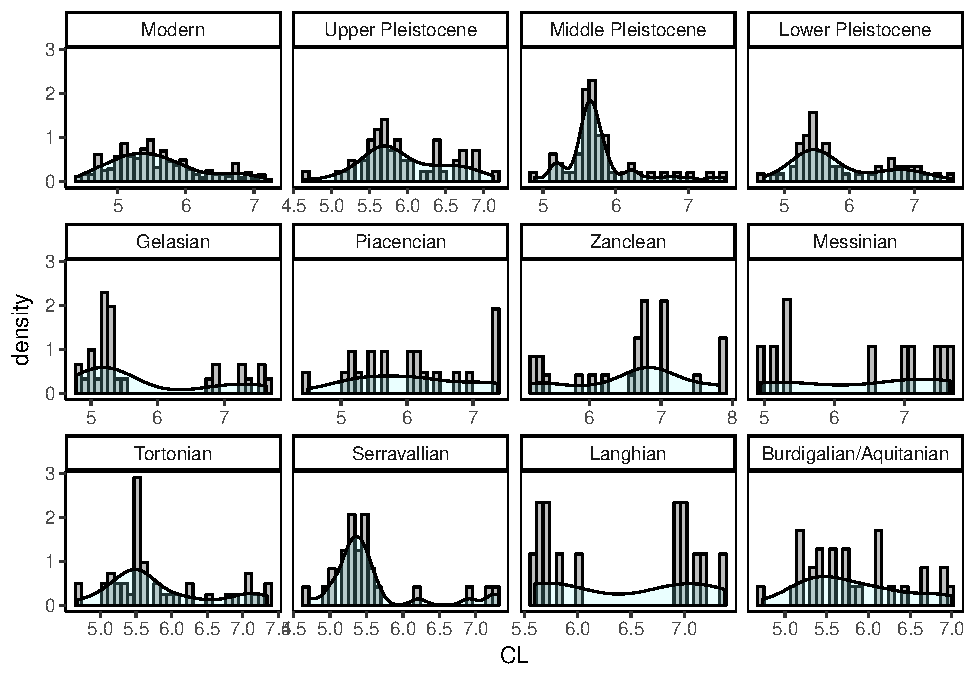
\includegraphics{MA_JJ_files/figure-latex/HistBins-1.pdf}
\caption{Distribution of body size data per time bin, logtransformed.}
\end{figure}

\newpage

\subsection{modern vs.~fossil}\label{modern-vs.fossil}

\begin{verbatim}
## `stat_bin()` using `bins = 30`. Pick better value with `binwidth`.
\end{verbatim}

\begin{figure}[htbp]
\centering
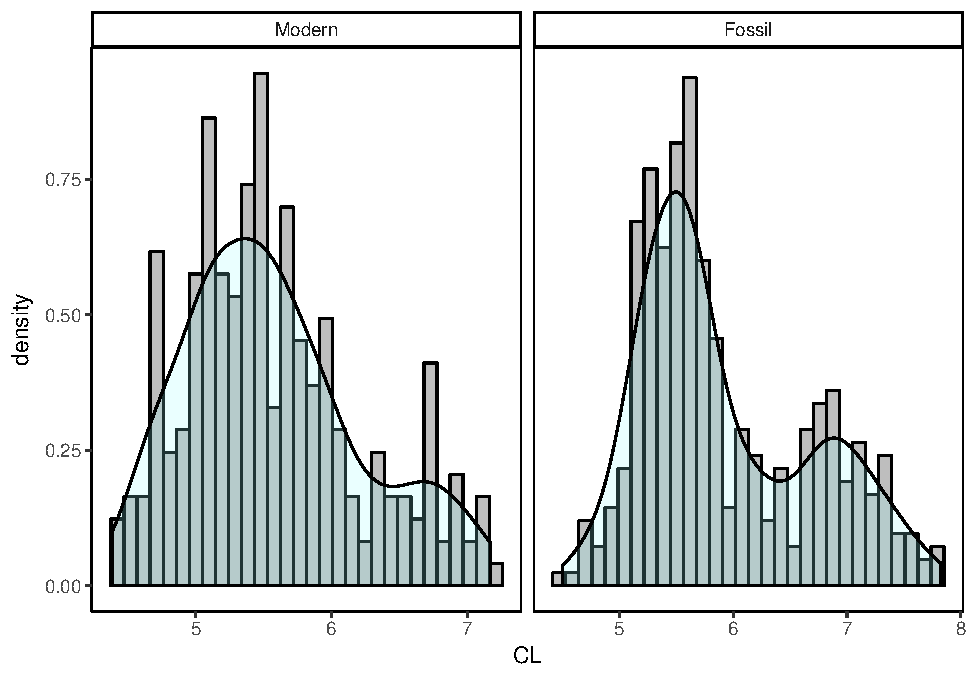
\includegraphics{MA_JJ_files/figure-latex/HistFosMo-1.pdf}
\caption{Distribution of body size data modern vs.~fossil,
logtransformed.}
\end{figure}

\newpage

\subsection{modern vs.~fossil, continental
vs.~insular}\label{modern-vs.fossil-continental-vs.insular}

\begin{verbatim}
## `stat_bin()` using `bins = 30`. Pick better value with `binwidth`.
\end{verbatim}

\begin{figure}[htbp]
\centering
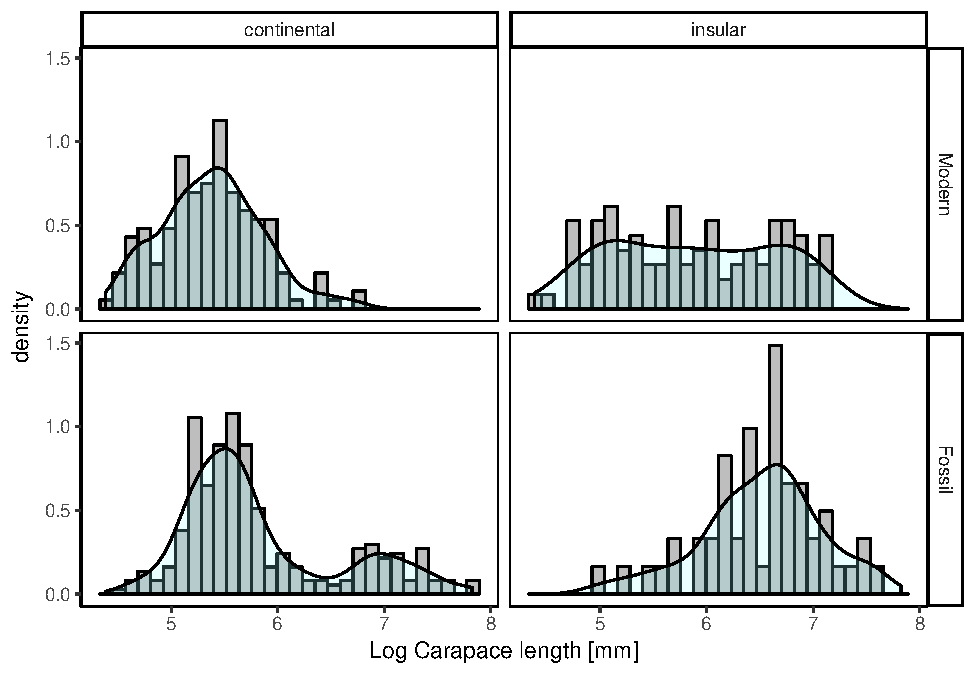
\includegraphics{MA_JJ_files/figure-latex/HistFMCI-1.pdf}
\caption{Distribution of body size data modern vs.~fossil, continental
vs.~insular logtransformed.}
\end{figure}

\newpage

\subsection{continental vs.~insular}\label{continental-vs.insular}

\begin{verbatim}
## `stat_bin()` using `bins = 30`. Pick better value with `binwidth`.
\end{verbatim}

\begin{figure}[htbp]
\centering
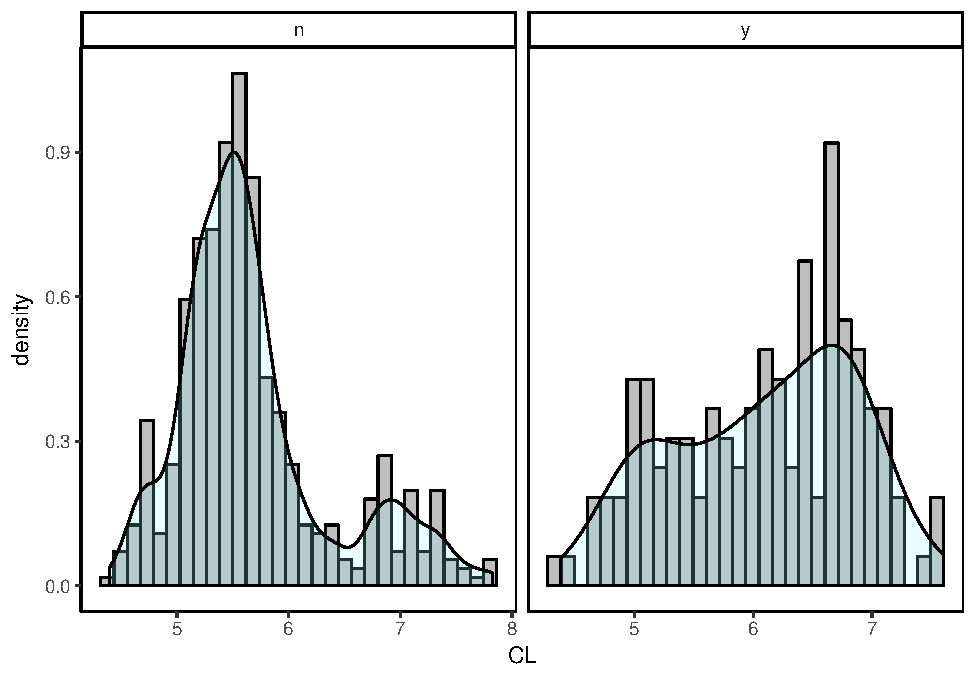
\includegraphics{MA_JJ_files/figure-latex/HistCI-1.pdf}
\caption{Distribution of body site data of continental (n) and
insular(y) species, logtransformed.}
\end{figure}

\newpage

\subsection{continents}\label{continents}

\begin{verbatim}
## `stat_bin()` using `bins = 30`. Pick better value with `binwidth`.
\end{verbatim}

\begin{figure}[htbp]
\centering
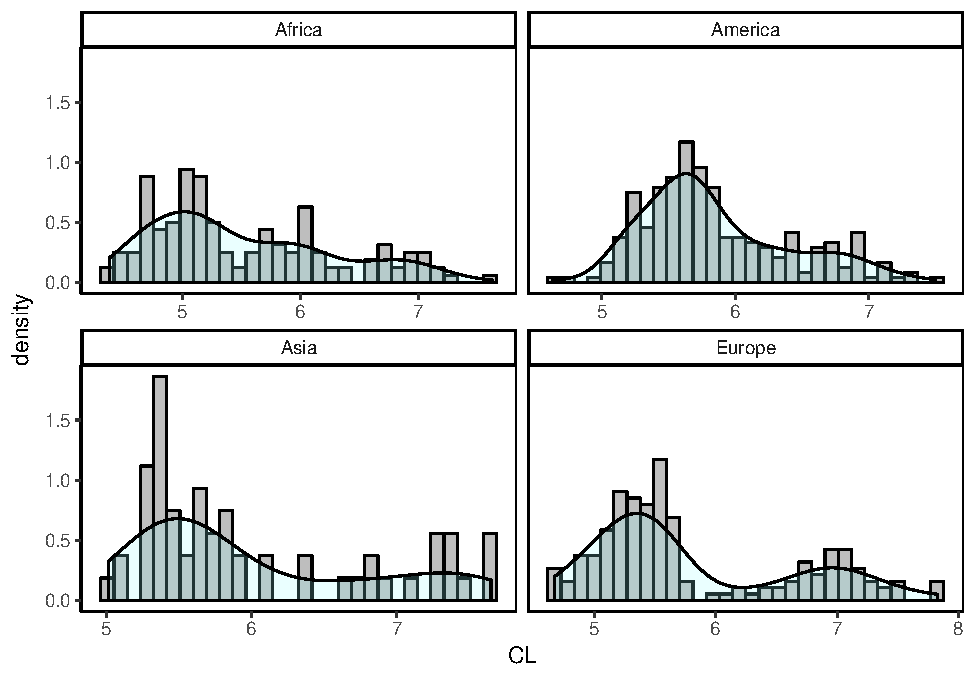
\includegraphics{MA_JJ_files/figure-latex/HistCon-1.pdf}
\caption{Distribution of body site data per continent, logtransformed.}
\end{figure}

\newpage

\subsection{General statistics}\label{general-statistics}

\begin{longtable}[]{@{}rrrrrrrrrrrrl@{}}
\caption{General statistics of body size data: all, per time bin,
insular and continental, per continent (all referring to CL: min, max,
variance, mean, logmean, median, logmedian, skewness, logskewness,
kurosis, logkurtosis}\tabularnewline
\toprule
nCL & min & max & var & mean & logm & med & logmed & skew & logsk & kurt
& logku & Variable\tabularnewline
\midrule
\endfirsthead
\toprule
nCL & min & max & var & mean & logm & med & logmed & skew & logsk & kurt
& logku & Variable\tabularnewline
\midrule
\endhead
616 & 80.00 & 2500 & 164537.80 & 437.2 & 2.5 & 270.5 & 2.4 & 2.14 & 0.69
& 8.00 & 2.73 & all\tabularnewline
253 & 80.00 & 1300 & 67485.50 & 330.3 & 2.4 & 242.0 & 2.4 & 1.83 & 0.58
& 5.87 & 2.69 & Modern\tabularnewline
49 & 102.44 & 1250 & 69690.66 & 445.9 & 2.6 & 334.7 & 2.5 & 1.20 & 0.24
& 3.61 & 2.56 & Upper Pleistocene\tabularnewline
53 & 132.00 & 1800 & 97910.83 & 387.1 & 2.5 & 292.9 & 2.5 & 3.03 & 1.52
& 12.24 & 5.55 & Middle Pleistocene\tabularnewline
57 & 107.80 & 2000 & 161948.82 & 463.5 & 2.5 & 263.0 & 2.4 & 1.74 & 0.73
& 5.76 & 2.40 & Lower Pleistocene\tabularnewline
31 & 118.90 & 2050 & 411224.51 & 555.2 & 2.5 & 194.9 & 2.3 & 1.31 & 0.93
& 3.12 & 2.11 & Gelasian\tabularnewline
21 & 90.00 & 1600 & 270535.82 & 610.6 & 2.6 & 428.0 & 2.6 & 1.00 & 0.14
& 2.50 & 1.99 & Piacencian\tabularnewline
26 & 176.00 & 2500 & 476162.71 & 955.2 & 2.9 & 857.5 & 2.9 & 1.11 &
-0.40 & 3.56 & 2.30 & Zanclean\tabularnewline
10 & 140.00 & 2100 & 602611.21 & 948.9 & 2.8 & 916.0 & 2.9 & 0.26 &
-0.22 & 1.49 & 1.29 & Messinian\tabularnewline
45 & 107.00 & 1540 & 175470.12 & 462.7 & 2.5 & 250.0 & 2.4 & 1.49 & 0.81
& 3.74 & 2.54 & Tortonian\tabularnewline
27 & 111.00 & 1500 & 126060.40 & 337.7 & 2.4 & 220.0 & 2.3 & 2.49 & 1.77
& 7.77 & 5.30 & Serravallian\tabularnewline
14 & 270.00 & 1600 & 230451.33 & 747.9 & 2.8 & 700.0 & 2.8 & 0.30 & 0.03
& 1.55 & 1.18 & Langhian\tabularnewline
30 & 113.00 & 1100 & 76288.76 & 406.8 & 2.5 & 302.4 & 2.5 & 1.27 & 0.45
& 3.45 & 2.26 & Burdigalian/Aquitanian\tabularnewline
253 & 80.00 & 1300 & 67485.50 & 330.3 & 2.4 & 242.0 & 2.4 & 1.83 & 0.58
& 5.87 & 2.69 & Modern\tabularnewline
363 & 90.00 & 2500 & 219004.66 & 511.7 & 2.6 & 285.6 & 2.5 & 1.83 & 0.68
& 6.11 & 2.42 & Fossil\tabularnewline
469 & 81.00 & 2500 & 157808.79 & 392.9 & 2.5 & 250.0 & 2.4 & 2.65 & 1.07
& 10.57 & 3.74 & continental\tabularnewline
147 & 80.00 & 2000 & 160834.35 & 578.5 & 2.6 & 500.0 & 2.7 & 1.02 &
-0.27 & 3.95 & 2.05 & insular\tabularnewline
157 & 81.00 & 830 & 17009.02 & 244.0 & 2.3 & 221.0 & 2.3 & 1.92 & 0.29 &
8.09 & 2.98 & modern-con\tabularnewline
96 & 80.00 & 1300 & 118641.09 & 471.5 & 2.6 & 353.0 & 2.5 & 0.82 & 0.01
& 2.47 & 1.77 & modern-ins\tabularnewline
312 & 90.00 & 2500 & 212116.79 & 467.9 & 2.5 & 270.0 & 2.4 & 2.11 & 0.96
& 7.25 & 2.96 & fossil-con\tabularnewline
51 & 150.00 & 2000 & 180825.40 & 780.0 & 2.8 & 750.0 & 2.9 & 1.11 &
-0.40 & 4.02 & 3.18 & fossil-ins\tabularnewline
142 & 80.00 & 2050 & 112417.26 & 347.7 & 2.4 & 193.5 & 2.3 & 2.10 & 0.68
& 7.97 & 2.48 & Africa\tabularnewline
242 & 102.44 & 1800 & 82209.71 & 415.0 & 2.5 & 302.2 & 2.5 & 1.92 & 0.75
& 6.79 & 2.91 & America\tabularnewline
59 & 150.00 & 2100 & 323123.20 & 585.5 & 2.6 & 280.0 & 2.4 & 1.43 & 0.85
& 3.61 & 2.24 & Asia\tabularnewline
173 & 107.00 & 2500 & 254222.84 & 491.2 & 2.5 & 245.0 & 2.4 & 1.86 &
0.81 & 6.30 & 2.34 & Europe\tabularnewline
\bottomrule
\end{longtable}

\newpage

\section{Boxplots}\label{boxplots}

\subsection{genera per time bins}\label{genera-per-time-bins}

\begin{figure}[htbp]
\centering
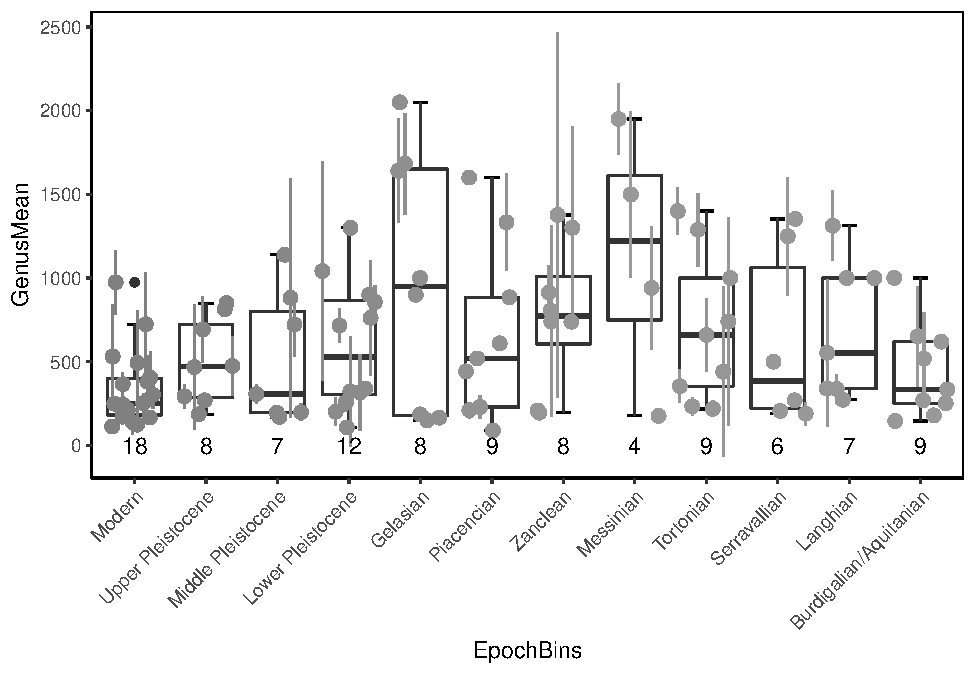
\includegraphics{MA_JJ_files/figure-latex/BPGBins-1.pdf}
\caption{Boxplots of mean CL per time bin, including mean and sd CL for
each genus (as pointrange).}
\end{figure}

\newpage

\subsection{continental vs.~insular per time
bin}\label{continental-vs.insular-per-time-bin}

\begin{figure}[htbp]
\centering
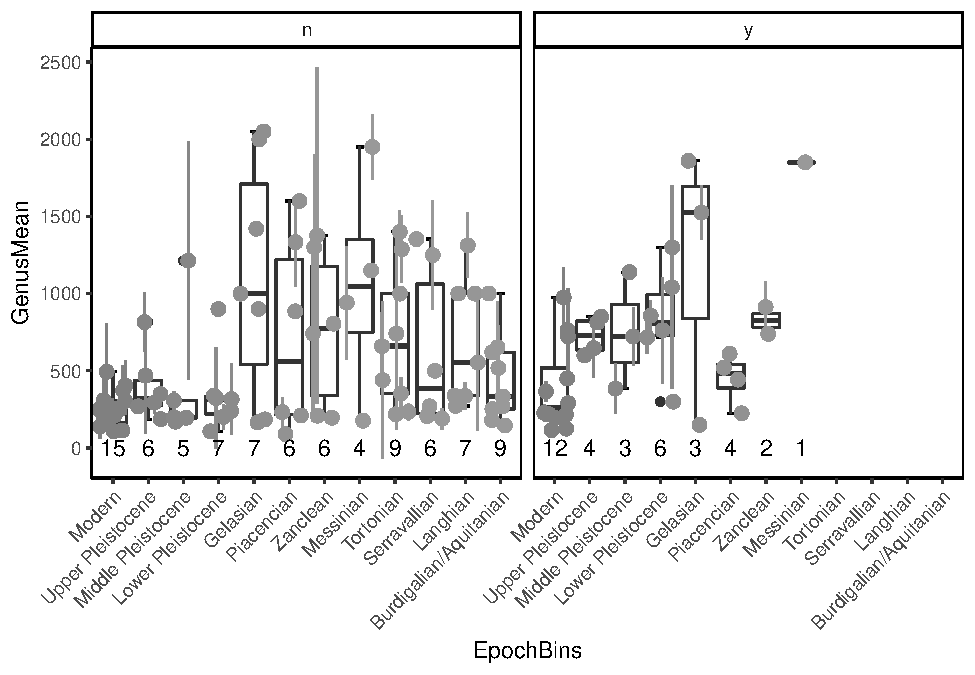
\includegraphics{MA_JJ_files/figure-latex/BPGBinsCI-1.pdf}
\caption{Boxplots of each genus per time bin, continental vs.~insular
species.}
\end{figure}

\newpage

\subsection{fossil vs.~modern}\label{fossil-vs.modern}

\begin{figure}[htbp]
\centering
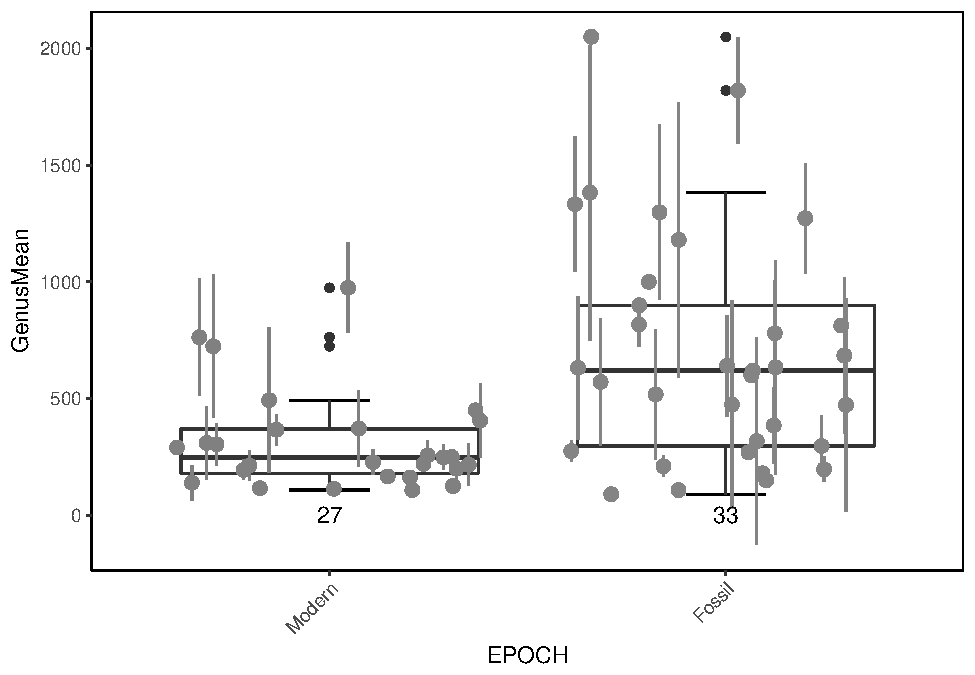
\includegraphics{MA_JJ_files/figure-latex/BPMF-1.pdf}
\caption{Boxplots fossil vs.~modern.}
\end{figure}

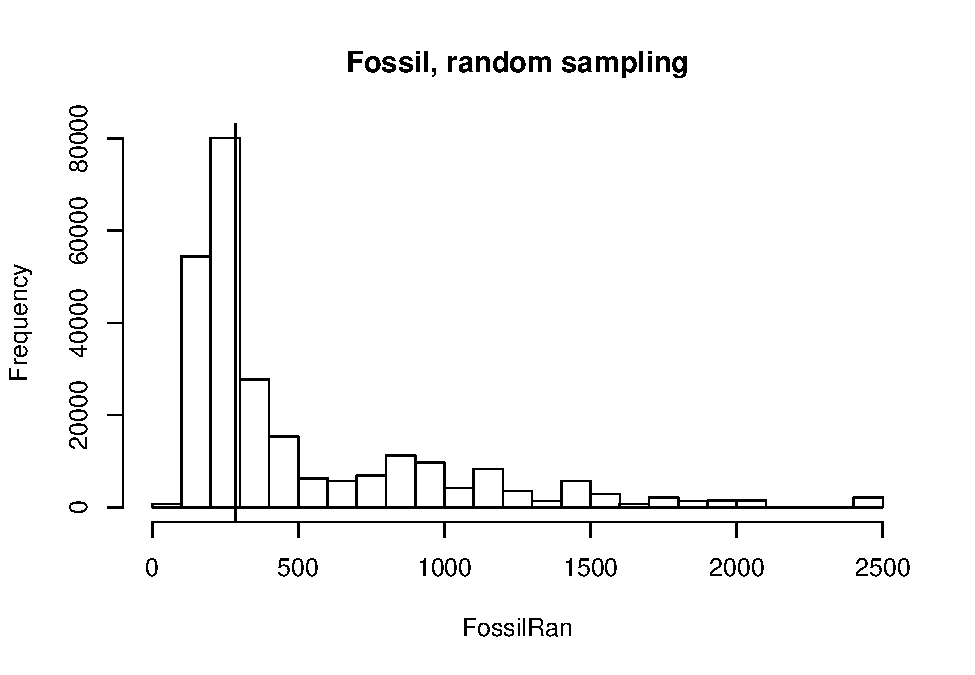
\includegraphics{MA_JJ_files/figure-latex/RSFM-1.pdf}

\begin{verbatim}
## [1] 330.3495
\end{verbatim}

\begin{verbatim}
## [1] 516.1724
\end{verbatim}

\begin{verbatim}
## 
##  Wilcoxon rank sum test with continuity correction
## 
## data:  Modern and Fossil
## W = 23372, p-value = 1.485e-07
## alternative hypothesis: true location shift is less than 0
\end{verbatim}

Wilcoxon Rank Sum Test (unpaired data):

modern \textless{} fossil (P = \(1.4850249\times 10^{-7}\))

\newpage

\subsection{fossil vs.~modern, continental
vs.~insular}\label{fossil-vs.modern-continental-vs.insular}

\begin{figure}[htbp]
\centering
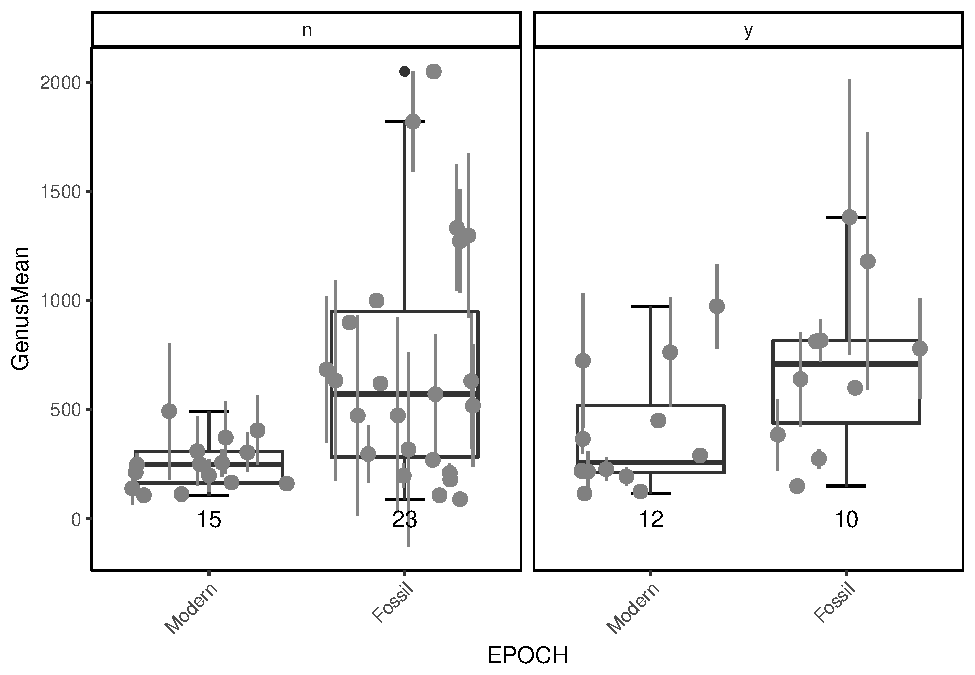
\includegraphics{MA_JJ_files/figure-latex/BPFMCI-1.pdf}
\caption{Boxplots fossil vs.~modern, continental vs.~insular species.}
\end{figure}

\begin{verbatim}
## [1] 51
\end{verbatim}

\begin{verbatim}
## [1] 51
\end{verbatim}

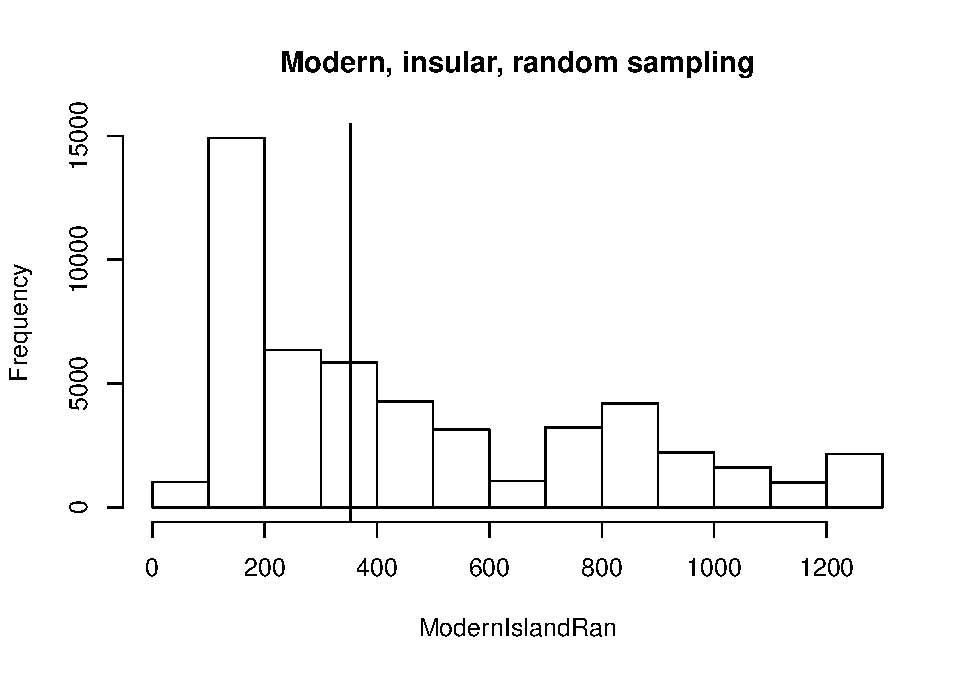
\includegraphics{MA_JJ_files/figure-latex/RSMFCI-1.pdf}

\begin{verbatim}
## 
##  Wilcoxon rank sum test with continuity correction
## 
## data:  ModernIsland and FossilIsland
## W = 730.5, p-value = 6.894e-05
## alternative hypothesis: true location shift is less than 0
\end{verbatim}

\begin{verbatim}
## [1] 157
\end{verbatim}

\begin{verbatim}
## [1] 157
\end{verbatim}

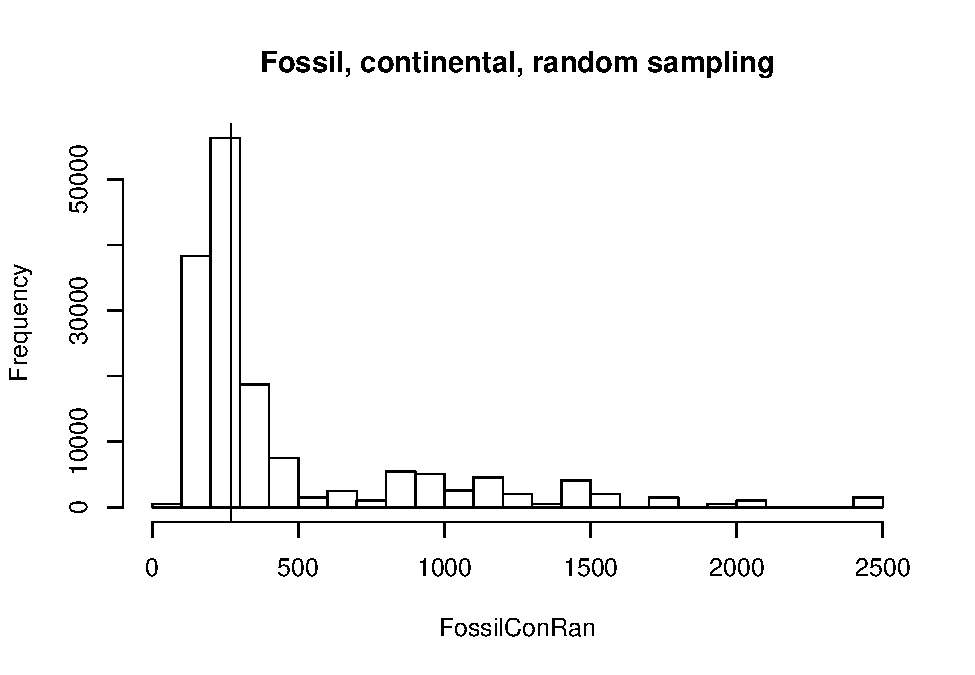
\includegraphics{MA_JJ_files/figure-latex/RSMFCI-2.pdf}

\begin{verbatim}
## 
##  Wilcoxon rank sum test with continuity correction
## 
## data:  ModernCon and FossilCon
## W = 8407, p-value = 5.589e-07
## alternative hypothesis: true location shift is less than 0
\end{verbatim}

Wilcoxon Rank Sum Test (unpaired data):

modern continental \textless{} fossil continental (P =
\(5.5894383\times 10^{-7}\))

modern insular \textless{} fossil insular (P =
\(6.8940531\times 10^{-5}\))

\newpage

\subsection{continental vs.~insular}\label{continental-vs.insular-1}

\begin{figure}[htbp]
\centering
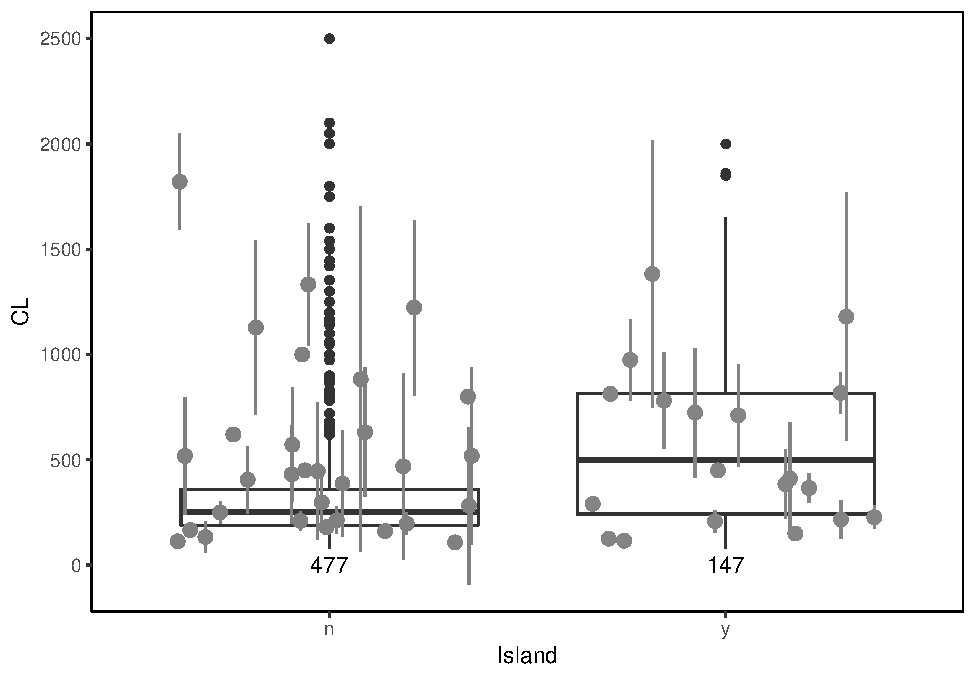
\includegraphics{MA_JJ_files/figure-latex/BPCI-1.pdf}
\caption{Boxplot continental vs.~insular, genera summarised}
\end{figure}

\begin{verbatim}
## [1] 147
\end{verbatim}

\begin{verbatim}
## [1] 147
\end{verbatim}

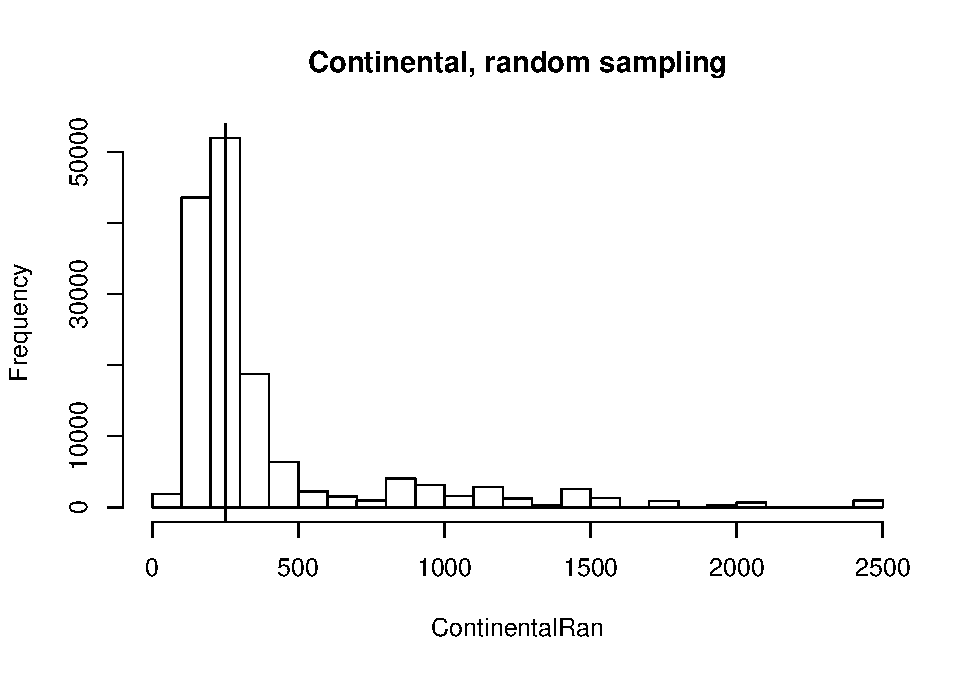
\includegraphics{MA_JJ_files/figure-latex/RSCI-1.pdf}

\begin{verbatim}
## 
##  Wilcoxon rank sum test with continuity correction
## 
## data:  Insular and Continental
## W = 13942, p-value = 8.407e-06
## alternative hypothesis: true location shift is greater than 0
\end{verbatim}

Wilcoxon Rank Sum Test (unpaired data):

continental \textless{} insular (P = \(8.4067298\times 10^{-6}\))

\newpage

\subsection{continental vs.~insular per time
bin}\label{continental-vs.insular-per-time-bin-1}

\begin{figure}[htbp]
\centering
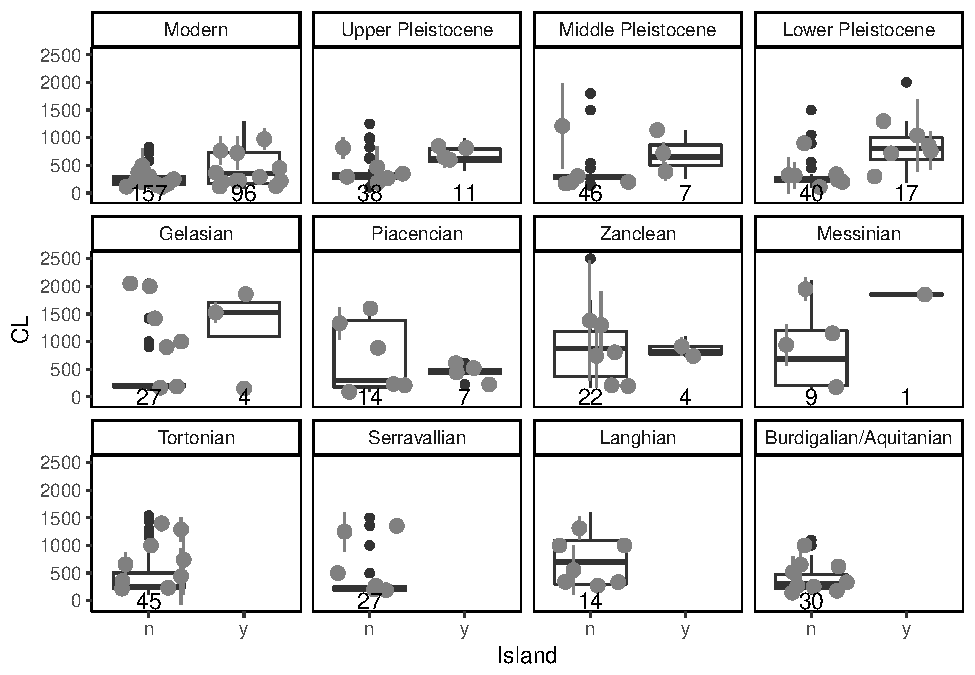
\includegraphics{MA_JJ_files/figure-latex/BPCIBins-1.pdf}
\caption{Boxplot continental vs.~insular, genera summarised}
\end{figure}

\newpage

\subsection{continents}\label{continents-1}

\begin{figure}[htbp]
\centering
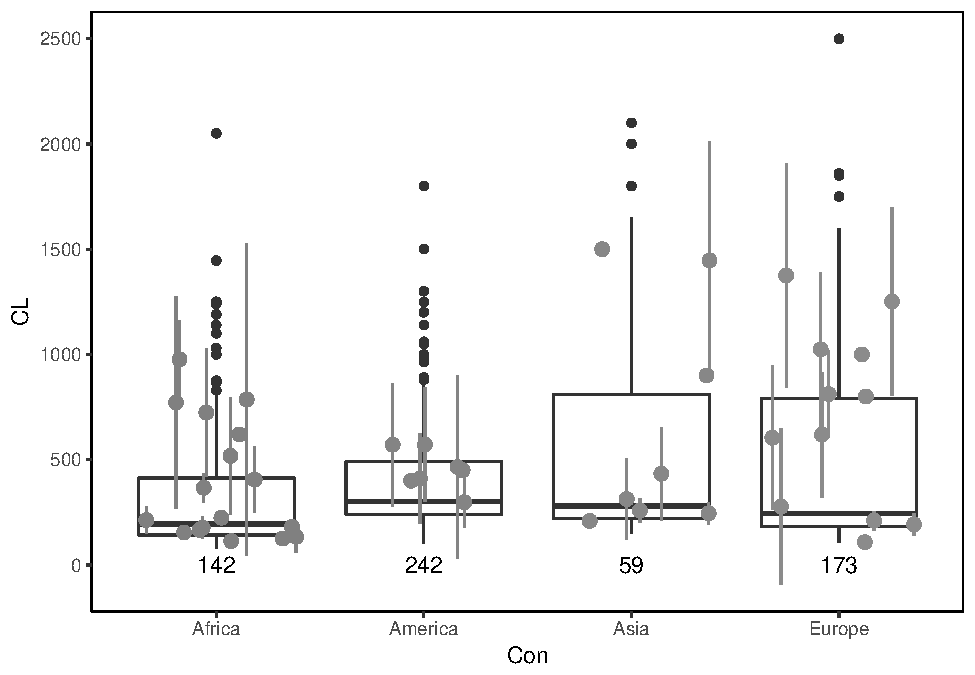
\includegraphics{MA_JJ_files/figure-latex/BPCon-1.pdf}
\caption{Boxplot: body size on different continents, genera summarised}
\end{figure}

\begin{verbatim}
## [1] 142
\end{verbatim}

\begin{verbatim}
## [1] 347.6887
\end{verbatim}

\begin{verbatim}
## [1] 142
\end{verbatim}

\begin{verbatim}
## [1] 399.0842
\end{verbatim}

\begin{verbatim}
## [1] 59
\end{verbatim}

\begin{verbatim}
## [1] 173
\end{verbatim}

\begin{verbatim}
## [1] 142
\end{verbatim}

\begin{verbatim}
## [1] 545.462
\end{verbatim}

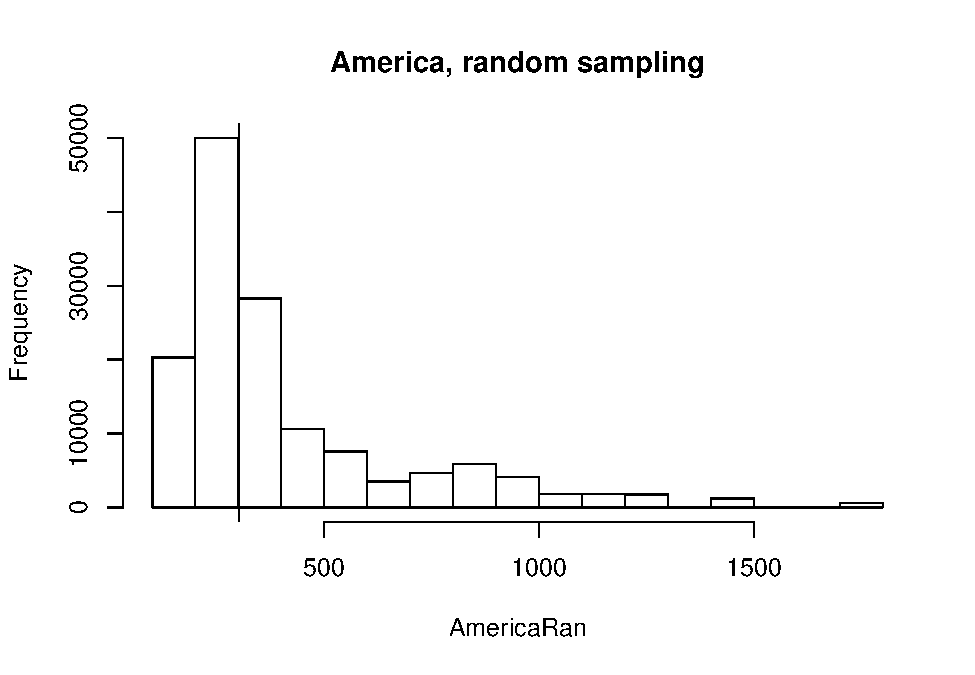
\includegraphics{MA_JJ_files/figure-latex/RSCon-1.pdf}
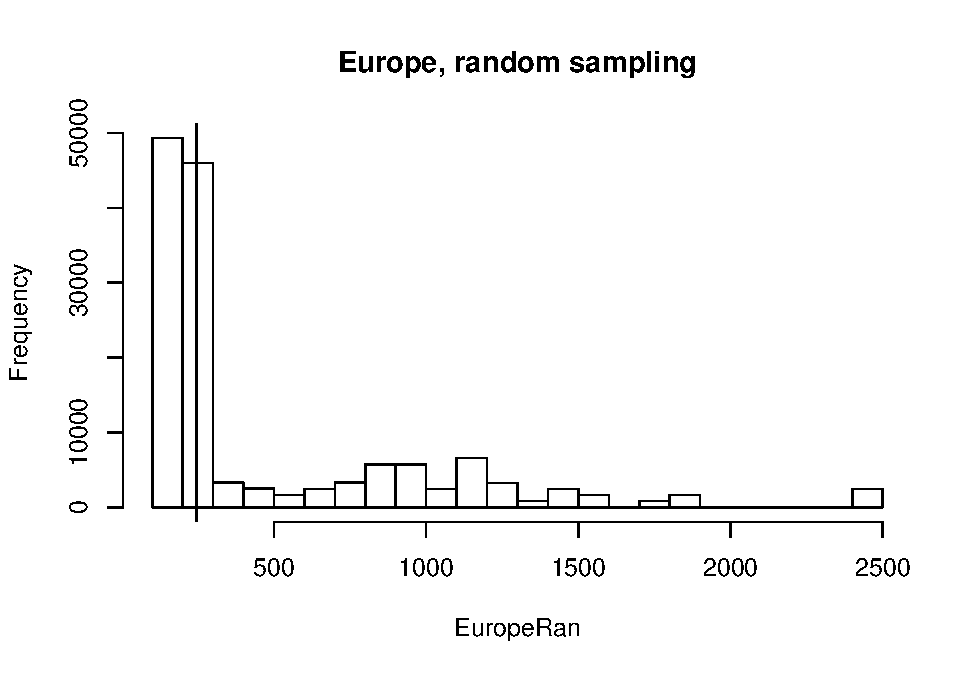
\includegraphics{MA_JJ_files/figure-latex/RSCon-2.pdf}
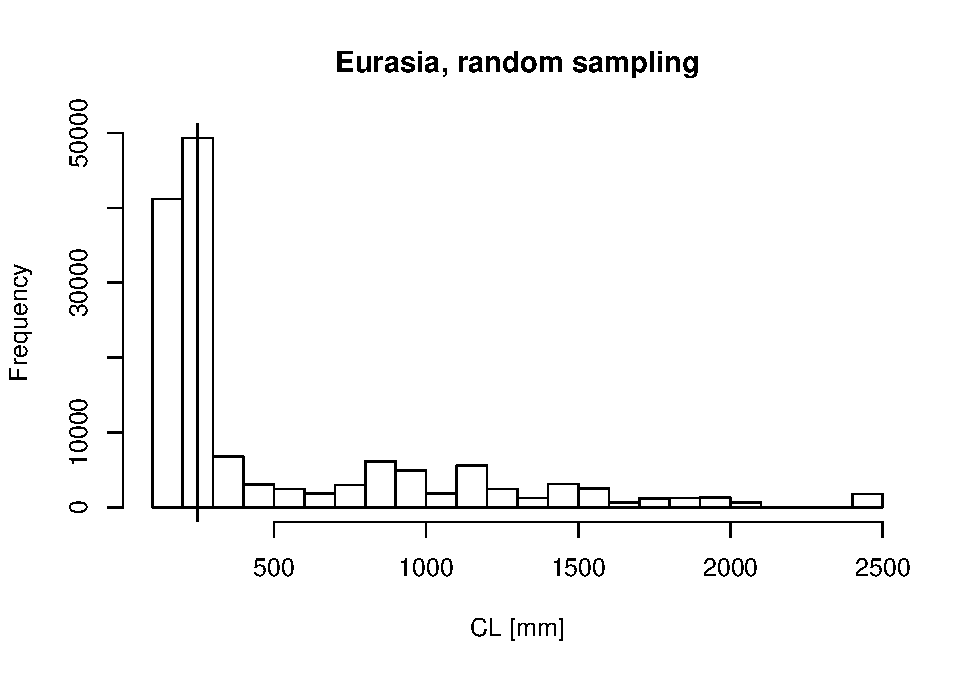
\includegraphics{MA_JJ_files/figure-latex/RSCon-3.pdf}

\begin{verbatim}
## 
##  Kruskal-Wallis rank sum test
## 
## data:  list(Africa, America, Eurasia, Europe)
## Kruskal-Wallis chi-squared = 27.699, df = 3, p-value = 4.201e-06
\end{verbatim}

Kruskal-Wallis-Test:

Continent means differ (P = \(4.2009248\times 10^{-6}\)) (still have to
look into the details\ldots{})

\newpage

\subsection{continents, continental
vs.~insular}\label{continents-continental-vs.insular}

\begin{figure}[htbp]
\centering
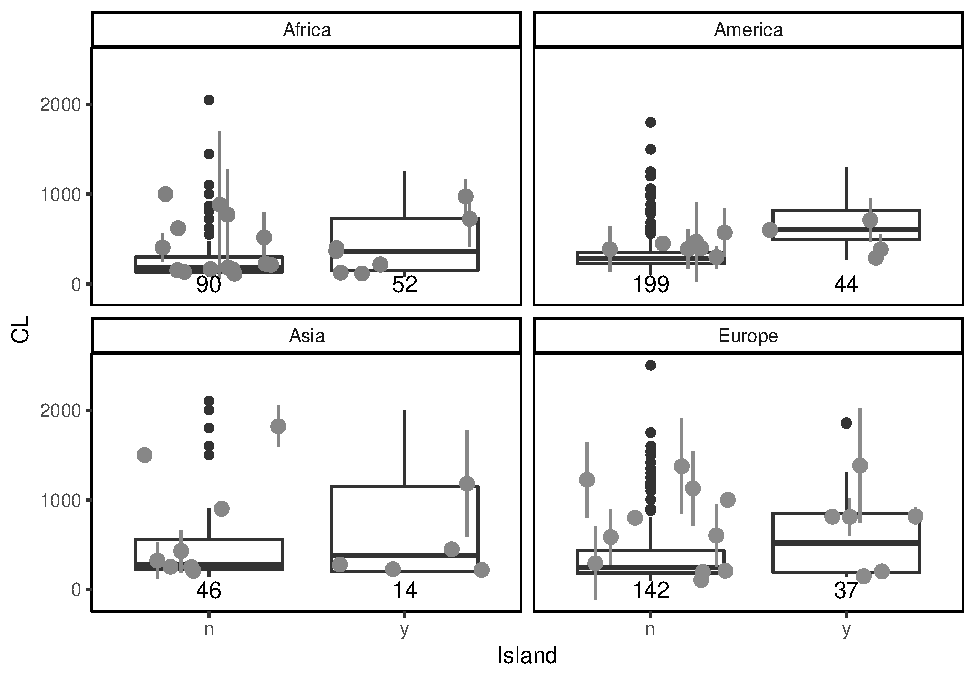
\includegraphics{MA_JJ_files/figure-latex/BPConCI-1.pdf}
\caption{Boxplot: body size on different continents, genera summarised}
\end{figure}

\newpage

\section{paleoTS analysis}\label{paleots-analysis}

\subsection{all (continental and
insular)}\label{all-continental-and-insular}

\subsubsection{genera (all)}\label{genera-all}

\begin{longtable}[]{@{}rrrr@{}}
\caption{paleoTS object, all data}\tabularnewline
\toprule
tt & mm & vv & nn\tabularnewline
\midrule
\endfirsthead
\toprule
tt & mm & vv & nn\tabularnewline
\midrule
\endhead
0.0000005 & 401.9641 & 102306.64 & 4\tabularnewline
0.0058500 & 314.1859 & 42607.58 & 18\tabularnewline
0.0688500 & 506.3265 & 64620.11 & 8\tabularnewline
0.4535000 & 516.4053 & 155241.85 & 7\tabularnewline
1.2935000 & 593.8669 & 147507.20 & 12\tabularnewline
2.1970000 & 971.8850 & 580540.76 & 8\tabularnewline
3.0940000 & 658.0826 & 271043.73 & 9\tabularnewline
4.4660000 & 785.0792 & 187937.61 & 8\tabularnewline
6.2890000 & 1141.9375 & 584378.85 & 4\tabularnewline
9.4270000 & 703.9570 & 195766.19 & 9\tabularnewline
12.7140000 & 628.3020 & 285258.36 & 6\tabularnewline
14.8950000 & 687.9619 & 169914.58 & 7\tabularnewline
19.5000000 & 441.5420 & 78467.65 & 9\tabularnewline
\bottomrule
\end{longtable}

\begin{figure}[htbp]
\centering
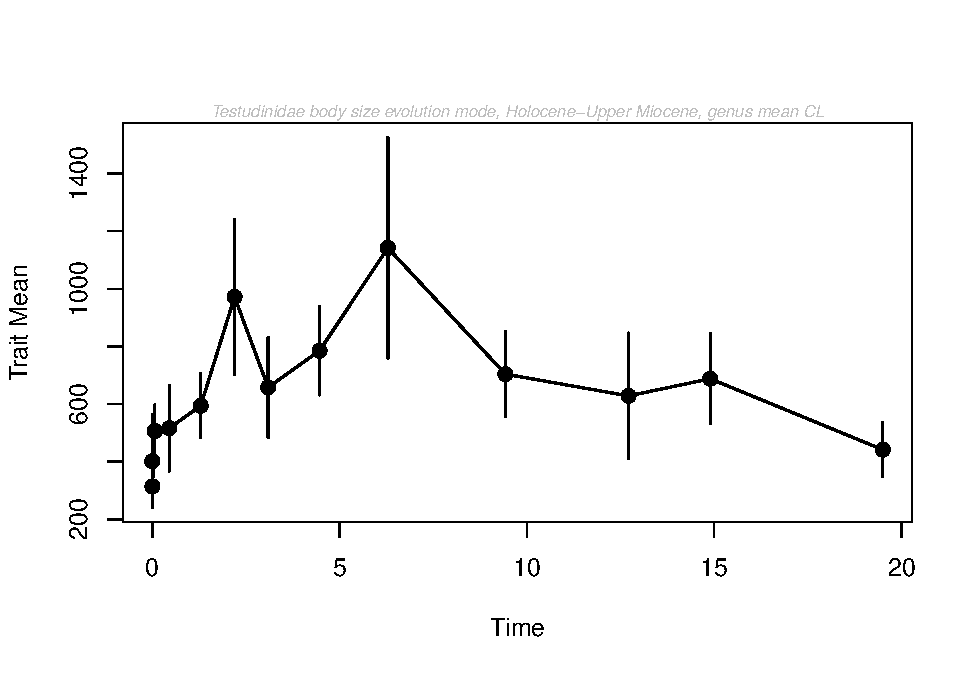
\includegraphics{MA_JJ_files/figure-latex/paleoTSAll-1.pdf}
\caption{paleoTS plot with genus mean, all}
\end{figure}

\begin{longtable}[]{@{}lrrrr@{}}
\caption{Model-fitting results for testudinidae, genera,
all}\tabularnewline
\toprule
& logL & K & AICc & Akaike.wt\tabularnewline
\midrule
\endfirsthead
\toprule
& logL & K & AICc & Akaike.wt\tabularnewline
\midrule
\endhead
GRW & -81.31790 & 2 & 167.9691 & 0.161\tabularnewline
URW & -82.05721 & 1 & 166.5144 & 0.332\tabularnewline
Stasis & -80.16802 & 2 & 165.6694 & 0.507\tabularnewline
\bottomrule
\end{longtable}

\newpage

\subsection{continental (excluding insular
species)}\label{continental-excluding-insular-species}

\subsubsection{genera (continental)}\label{genera-continental}

\begin{longtable}[]{@{}rrrr@{}}
\caption{paleoTS object, continental}\tabularnewline
\toprule
tt & mm & vv & nn\tabularnewline
\midrule
\endfirsthead
\toprule
tt & mm & vv & nn\tabularnewline
\midrule
\endhead
0.0000005 & 233.1680 & 8331.753 & 3\tabularnewline
0.0058500 & 241.7917 & 13004.928 & 15\tabularnewline
0.0688500 & 397.4606 & 50619.392 & 6\tabularnewline
0.4535000 & 416.9341 & 200982.124 & 5\tabularnewline
1.2935000 & 346.8484 & 66240.066 & 7\tabularnewline
2.1970000 & 1103.1067 & 595507.933 & 7\tabularnewline
3.0940000 & 725.4156 & 414253.291 & 6\tabularnewline
4.4660000 & 771.3833 & 259173.082 & 6\tabularnewline
6.2890000 & 1054.4375 & 531455.932 & 4\tabularnewline
9.4270000 & 703.9570 & 195766.185 & 9\tabularnewline
12.7140000 & 628.3020 & 285258.362 & 6\tabularnewline
14.8950000 & 687.9619 & 169914.577 & 7\tabularnewline
19.5000000 & 441.5420 & 78467.646 & 9\tabularnewline
\bottomrule
\end{longtable}

\begin{figure}[htbp]
\centering
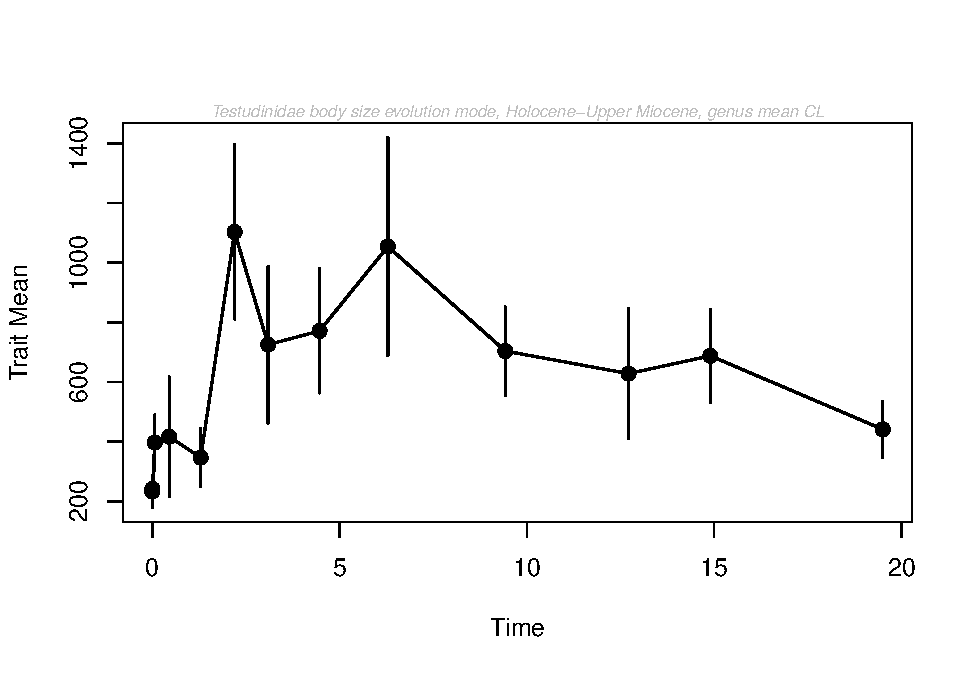
\includegraphics{MA_JJ_files/figure-latex/paleoTSC-1.pdf}
\caption{paleoTS plot with genus mean, continental}
\end{figure}

\begin{longtable}[]{@{}lrrrr@{}}
\caption{Model-fitting results for testudinidae, genera,
continental}\tabularnewline
\toprule
& logL & K & AICc & Akaike.wt\tabularnewline
\midrule
\endfirsthead
\toprule
& logL & K & AICc & Akaike.wt\tabularnewline
\midrule
\endhead
GRW & -82.26287 & 2 & 169.8591 & 0.300\tabularnewline
URW & -83.12577 & 1 & 168.6515 & 0.548\tabularnewline
Stasis & -82.93984 & 2 & 171.2130 & 0.152\tabularnewline
\bottomrule
\end{longtable}

\newpage

\subsection{insular (excluding
continental)}\label{insular-excluding-continental}

\subsubsection{genera (insular)}\label{genera-insular}

\begin{longtable}[]{@{}rrrr@{}}
\caption{paleoTS object, insular}\tabularnewline
\toprule
tt & mm & vv & nn\tabularnewline
\midrule
\endfirsthead
\toprule
tt & mm & vv & nn\tabularnewline
\midrule
\endhead
0.0000005 & 860.9268 & 0.00 & 1\tabularnewline
0.0058500 & 379.5354 & 68570.44 & 12\tabularnewline
0.0688500 & 727.5938 & 14997.58 & 4\tabularnewline
0.4535000 & 748.8333 & 142649.08 & 3\tabularnewline
1.2935000 & 829.6744 & 112964.44 & 6\tabularnewline
2.1970000 & 1178.3333 & 821158.33 & 3\tabularnewline
3.0940000 & 449.4375 & 27058.77 & 4\tabularnewline
4.4660000 & 826.1667 & 15196.06 & 2\tabularnewline
6.2890000 & 1850.0000 & 0.00 & 1\tabularnewline
\bottomrule
\end{longtable}

\begin{figure}[htbp]
\centering
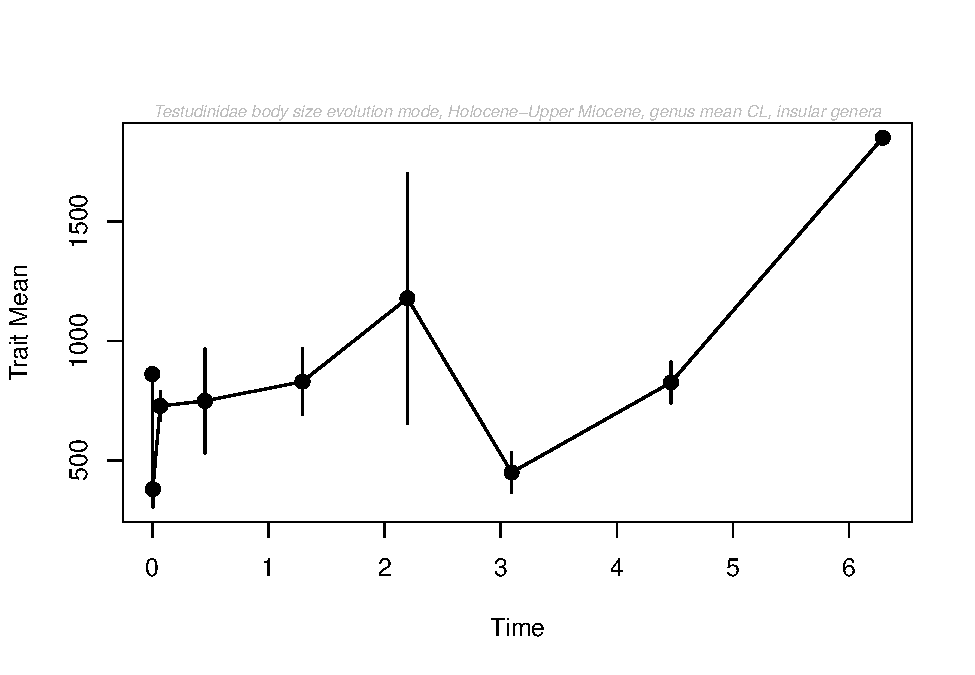
\includegraphics{MA_JJ_files/figure-latex/paleoTSI-1.pdf}
\caption{paleoTS plot with genus mean, insular}
\end{figure}

\begin{longtable}[]{@{}lrrrr@{}}
\caption{Model-fitting results for testudinidae, genera,
insular}\tabularnewline
\toprule
& logL & K & AICc & Akaike.wt\tabularnewline
\midrule
\endfirsthead
\toprule
& logL & K & AICc & Akaike.wt\tabularnewline
\midrule
\endhead
GRW & -68.57344 & 2 & 143.5469 & 0\tabularnewline
URW & -75.76576 & 1 & 154.1982 & 0\tabularnewline
Stasis & -60.41581 & 2 & 127.2316 & 1\tabularnewline
\bottomrule
\end{longtable}

\newpage

\subsection{per continent}\label{per-continent}

\subsubsection{Europe, genera}\label{europe-genera}

\begin{longtable}[]{@{}rrrr@{}}
\caption{paleoTS object, Europe}\tabularnewline
\toprule
mm & nn & vv & tt\tabularnewline
\midrule
\endfirsthead
\toprule
mm & nn & vv & tt\tabularnewline
\midrule
\endhead
148.8559 & 2 & 3338.406 & 0.00585\tabularnewline
616.6667 & 3 & 138802.333 & 0.06885\tabularnewline
377.8167 & 3 & 89203.953 & 0.45350\tabularnewline
697.3717 & 5 & 218431.974 & 1.29350\tabularnewline
895.0000 & 2 & 1110050.000 & 2.19700\tabularnewline
453.3333 & 3 & 39433.333 & 3.09400\tabularnewline
1215.8667 & 5 & 159317.256 & 4.46600\tabularnewline
838.3750 & 2 & 875495.281 & 6.28900\tabularnewline
800.0508 & 6 & 263434.389 & 9.42700\tabularnewline
653.9625 & 5 & 351634.528 & 12.71400\tabularnewline
772.0000 & 5 & 223154.375 & 14.89500\tabularnewline
533.8533 & 5 & 183706.682 & 19.50000\tabularnewline
\bottomrule
\end{longtable}

\begin{figure}[htbp]
\centering
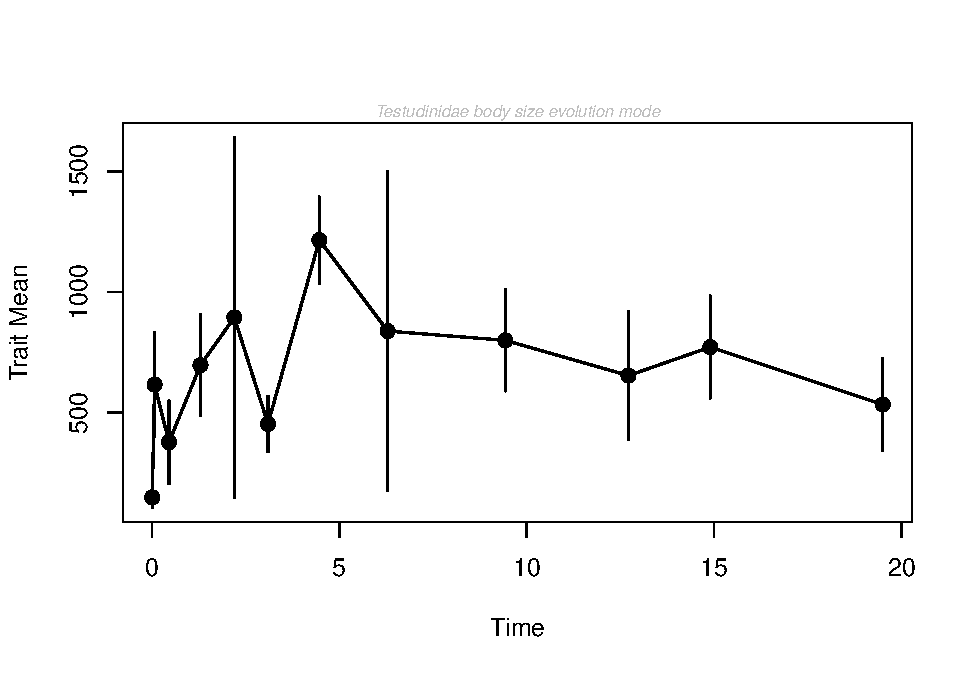
\includegraphics{MA_JJ_files/figure-latex/paleoTSEurope-1.pdf}
\caption{Genera, Europe}
\end{figure}

\begin{longtable}[]{@{}lrrrr@{}}
\caption{Model-fitting results for testudinidae, genera,
Europe}\tabularnewline
\toprule
& logL & K & AICc & Akaike.wt\tabularnewline
\midrule
\endfirsthead
\toprule
& logL & K & AICc & Akaike.wt\tabularnewline
\midrule
\endhead
GRW & -84.14010 & 2 & 173.7802 & 0.006\tabularnewline
URW & -85.90727 & 1 & 174.2590 & 0.005\tabularnewline
Stasis & -79.01365 & 2 & 163.5273 & 0.990\tabularnewline
\bottomrule
\end{longtable}

\newpage

\paragraph{Europe, smaller original bins (see Table 2), genera,
continental}\label{europe-smaller-original-bins-see-table-2-genera-continental}

\begin{longtable}[]{@{}rrrr@{}}
\caption{paleoTs object, Europe, continental}\tabularnewline
\toprule
mm & nn & vv & tt\tabularnewline
\midrule
\endfirsthead
\toprule
mm & nn & vv & tt\tabularnewline
\midrule
\endhead
149.5381 & 2 & 3450.8267 & 0.00585\tabularnewline
187.0000 & 1 & 0.0000 & 0.06885\tabularnewline
205.4750 & 2 & 198.0050 & 0.45350\tabularnewline
204.9292 & 2 & 23.1767 & 1.29350\tabularnewline
1420.0000 & 1 & 0.0000 & 2.19700\tabularnewline
232.5000 & 1 & 0.0000 & 3.09400\tabularnewline
1475.6667 & 3 & 57926.3333 & 4.46600\tabularnewline
663.3750 & 2 & 473607.7812 & 6.28900\tabularnewline
800.0508 & 6 & 263434.3893 & 9.42700\tabularnewline
653.9625 & 5 & 351634.5281 & 12.71400\tabularnewline
772.0000 & 5 & 223154.3750 & 14.89500\tabularnewline
533.8533 & 5 & 183706.6821 & 19.50000\tabularnewline
\bottomrule
\end{longtable}

\begin{figure}[htbp]
\centering
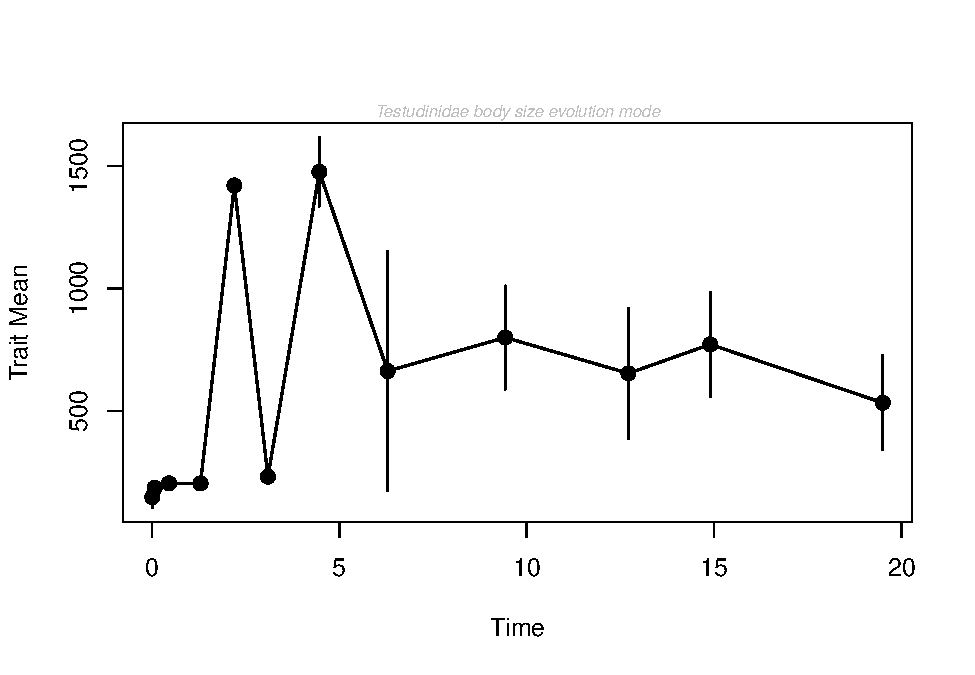
\includegraphics{MA_JJ_files/figure-latex/pTSEuC-1.pdf}
\caption{paleoTS, genera, Europe, continental}
\end{figure}

\begin{longtable}[]{@{}lrrrr@{}}
\caption{Model-fitting results for testudinidae, genera, Europe,
continental}\tabularnewline
\toprule
& logL & K & AICc & Akaike.wt\tabularnewline
\midrule
\endfirsthead
\toprule
& logL & K & AICc & Akaike.wt\tabularnewline
\midrule
\endhead
GRW & -87.93137 & 2 & 181.3627 & 0.009\tabularnewline
URW & -92.56882 & 1 & 187.5821 & 0.000\tabularnewline
Stasis & -83.21073 & 2 & 171.9215 & 0.991\tabularnewline
\bottomrule
\end{longtable}

\newpage

\paragraph{Europe, smaller original bins (see Table 2), genera,
insular}\label{europe-smaller-original-bins-see-table-2-genera-insular}

\begin{longtable}[]{@{}rrrr@{}}
\caption{paleoTs object, Europe, insular}\tabularnewline
\toprule
mm & nn & vv & tt\tabularnewline
\midrule
\endfirsthead
\toprule
mm & nn & vv & tt\tabularnewline
\midrule
\endhead
187.5077 & 1 & 0.00 & 0.00585\tabularnewline
831.5000 & 2 & 684.50 & 0.06885\tabularnewline
722.5000 & 1 & 0.00 & 0.45350\tabularnewline
835.0833 & 4 & 168423.36 & 1.29350\tabularnewline
1005.0000 & 2 & 1462050.00 & 2.19700\tabularnewline
451.6667 & 3 & 40558.33 & 3.09400\tabularnewline
826.1667 & 2 & 15196.06 & 4.46600\tabularnewline
1850.0000 & 1 & 0.00 & 6.28900\tabularnewline
\bottomrule
\end{longtable}

\begin{figure}[htbp]
\centering
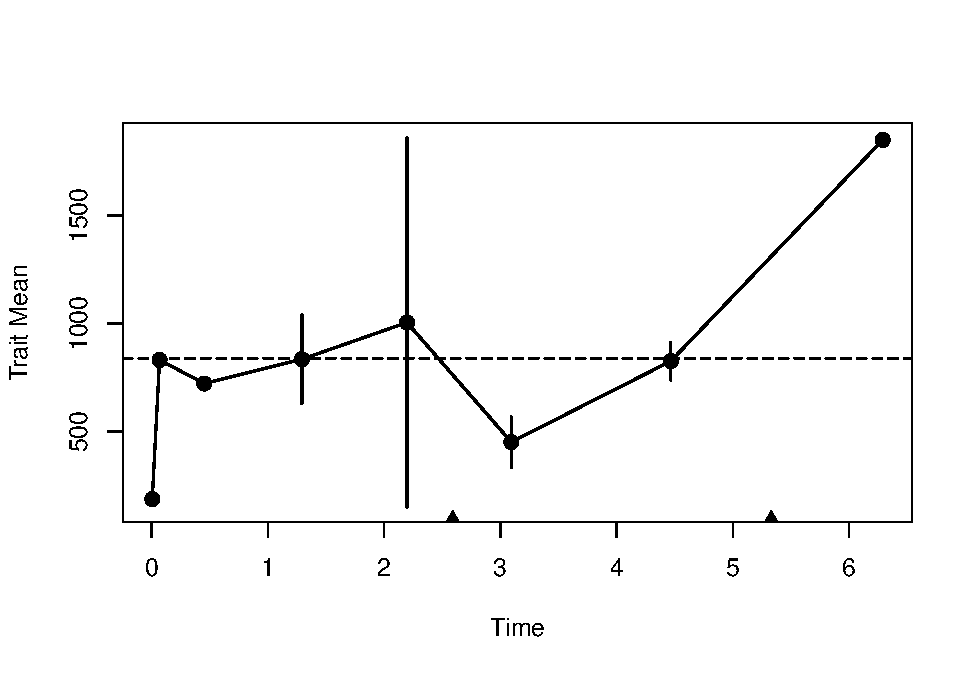
\includegraphics{MA_JJ_files/figure-latex/pTSEuI-1.pdf}
\caption{paleoTS, genera, Europe, insular}
\end{figure}

\begin{longtable}[]{@{}lrrrr@{}}
\caption{Model-fitting results for testudinidae, genera, Europe,
insular}\tabularnewline
\toprule
& logL & K & AICc & Akaike.wt\tabularnewline
\midrule
\endfirsthead
\toprule
& logL & K & AICc & Akaike.wt\tabularnewline
\midrule
\endhead
GRW & -67.12192 & 2 & 141.2438 & 0.000\tabularnewline
URW & -57.51634 & 1 & 117.8327 & 0.074\tabularnewline
Stasis & -52.89638 & 2 & 112.7928 & 0.926\tabularnewline
\bottomrule
\end{longtable}

\newpage 

\subsubsection{Eurasia, smaller original bins (See Table 2),
genera}\label{eurasia-smaller-original-bins-see-table-2-genera}

\begin{longtable}[]{@{}rrrr@{}}
\caption{paleoTS object, Eurasia}\tabularnewline
\toprule
tt & mm & vv & nn\tabularnewline
\midrule
\endfirsthead
\toprule
tt & mm & vv & nn\tabularnewline
\midrule
\endhead
0.0000005 & 137.2637 & 0.000 & 1\tabularnewline
0.0058500 & 236.8217 & 9760.467 & 5\tabularnewline
0.0688500 & 530.0000 & 122579.333 & 4\tabularnewline
0.4535000 & 377.8167 & 89203.953 & 3\tabularnewline
1.2935000 & 777.5579 & 162641.142 & 7\tabularnewline
2.1970000 & 909.6667 & 562217.222 & 5\tabularnewline
3.0940000 & 892.0000 & 381770.000 & 5\tabularnewline
4.4660000 & 1048.0556 & 296417.219 & 6\tabularnewline
6.2890000 & 1208.9167 & 849651.021 & 3\tabularnewline
9.4270000 & 800.0508 & 263434.389 & 6\tabularnewline
12.7140000 & 653.9625 & 351634.528 & 5\tabularnewline
14.8950000 & 772.0000 & 223154.375 & 5\tabularnewline
19.5000000 & 513.8533 & 162399.349 & 5\tabularnewline
\bottomrule
\end{longtable}

\begin{figure}[htbp]
\centering
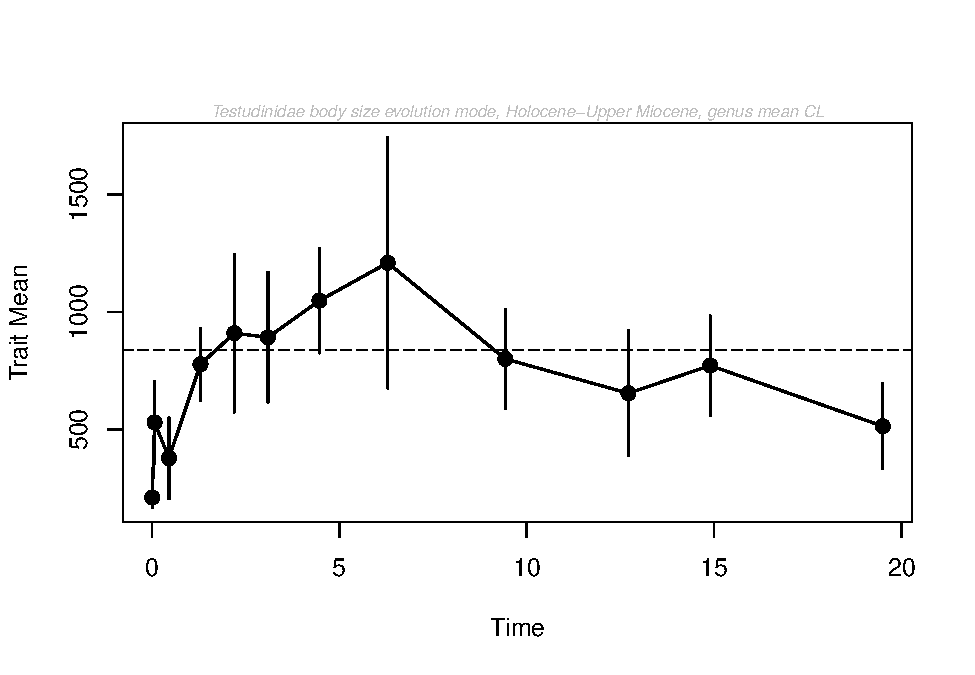
\includegraphics{MA_JJ_files/figure-latex/paleoTSEurasia-1.pdf}
\caption{paleoTS, genera, Eurasia}
\end{figure}

\begin{longtable}[]{@{}lrrrr@{}}
\caption{Model-fitting results for testudinidae, genera,
Eurasia}\tabularnewline
\toprule
& logL & K & AICc & Akaike.wt\tabularnewline
\midrule
\endfirsthead
\toprule
& logL & K & AICc & Akaike.wt\tabularnewline
\midrule
\endhead
GRW & -85.25195 & 2 & 175.8372 & 0.149\tabularnewline
URW & -85.39072 & 1 & 173.1814 & 0.562\tabularnewline
Stasis & -84.58890 & 2 & 174.5111 & 0.289\tabularnewline
\bottomrule
\end{longtable}

\newpage 

\subsubsection{Eurasia, smaller original bins (See Table 2), genera,
continental}\label{eurasia-smaller-original-bins-see-table-2-genera-continental}

\begin{longtable}[]{@{}rrrr@{}}
\caption{paleoTS object, Eurasia, continental}\tabularnewline
\toprule
tt & mm & vv & nn\tabularnewline
\midrule
\endfirsthead
\toprule
tt & mm & vv & nn\tabularnewline
\midrule
\endhead
0.0000005 & 137.2637 & 0.000 & 1\tabularnewline
0.0058500 & 238.0120 & 9654.865 & 5\tabularnewline
0.0688500 & 228.5000 & 3444.500 & 2\tabularnewline
0.4535000 & 205.4750 & 198.005 & 2\tabularnewline
1.2935000 & 595.5388 & 191487.404 & 4\tabularnewline
2.1970000 & 1044.5833 & 442006.250 & 4\tabularnewline
3.0940000 & 1110.8333 & 581102.083 & 3\tabularnewline
4.4660000 & 1159.0000 & 439728.667 & 4\tabularnewline
6.2890000 & 1092.2500 & 788605.188 & 3\tabularnewline
9.4270000 & 800.0508 & 263434.389 & 6\tabularnewline
12.7140000 & 653.9625 & 351634.528 & 5\tabularnewline
14.8950000 & 772.0000 & 223154.375 & 5\tabularnewline
19.5000000 & 513.8533 & 162399.349 & 5\tabularnewline
\bottomrule
\end{longtable}

\begin{figure}[htbp]
\centering
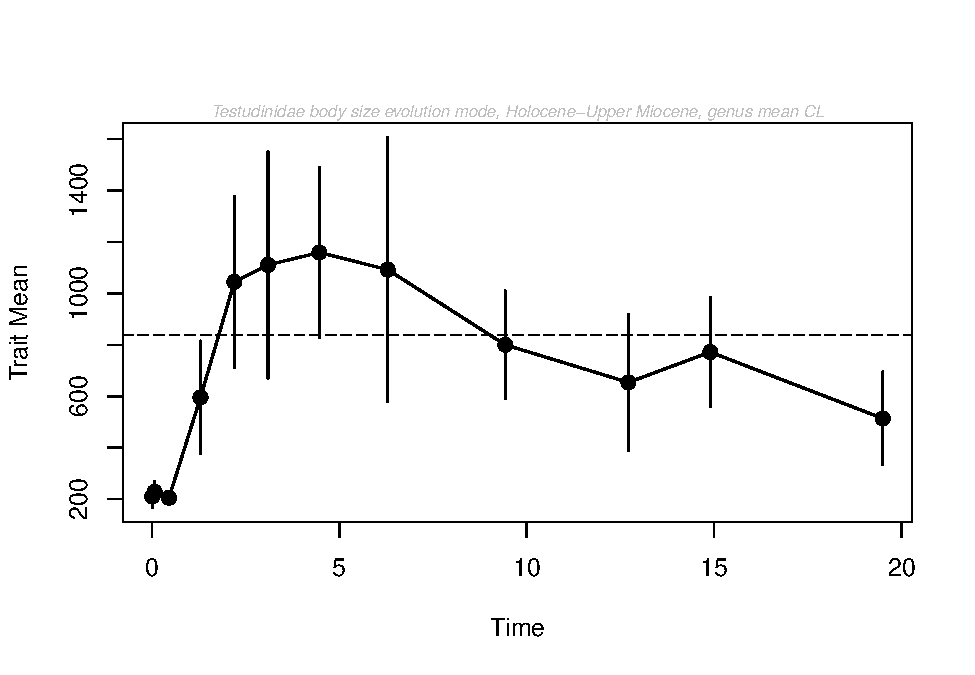
\includegraphics{MA_JJ_files/figure-latex/pTSEsC-1.pdf}
\caption{paleoTS, genera, Eurasia, continental}
\end{figure}

\begin{longtable}[]{@{}lrrrr@{}}
\caption{Model-fitting results for testudinidae, genera, Eurasia,
continental}\tabularnewline
\toprule
& logL & K & AICc & Akaike.wt\tabularnewline
\midrule
\endfirsthead
\toprule
& logL & K & AICc & Akaike.wt\tabularnewline
\midrule
\endhead
GRW & -82.20698 & 2 & 169.7473 & 0.222\tabularnewline
URW & -82.42344 & 1 & 167.2469 & 0.776\tabularnewline
Stasis & -87.19538 & 2 & 179.7241 & 0.002\tabularnewline
\bottomrule
\end{longtable}

\newpage 

\subsubsection{Eurasia, smaller original bins (See Table 2), genera,
insular}\label{eurasia-smaller-original-bins-see-table-2-genera-insular}

\begin{longtable}[]{@{}rrrr@{}}
\caption{paleoTS object, Eurasia, insular}\tabularnewline
\toprule
tt & mm & vv & nn\tabularnewline
\midrule
\endfirsthead
\toprule
tt & mm & vv & nn\tabularnewline
\midrule
\endhead
0.0000005 & 137.2637 & 0.000 & 1\tabularnewline
0.0058500 & 271.4596 & 5668.485 & 4\tabularnewline
0.0688500 & 644.3333 & 105436.333 & 3\tabularnewline
0.4535000 & 722.5000 & 0.000 & 1\tabularnewline
1.2935000 & 882.0356 & 105684.077 & 6\tabularnewline
2.1970000 & 953.6667 & 652233.889 & 5\tabularnewline
3.0940000 & 891.0000 & 383430.000 & 5\tabularnewline
4.4660000 & 620.4444 & 134562.926 & 3\tabularnewline
6.2890000 & 1900.0000 & 5000.000 & 2\tabularnewline
19.5000000 & 800.0000 & 0.000 & 1\tabularnewline
\bottomrule
\end{longtable}

\begin{figure}[htbp]
\centering
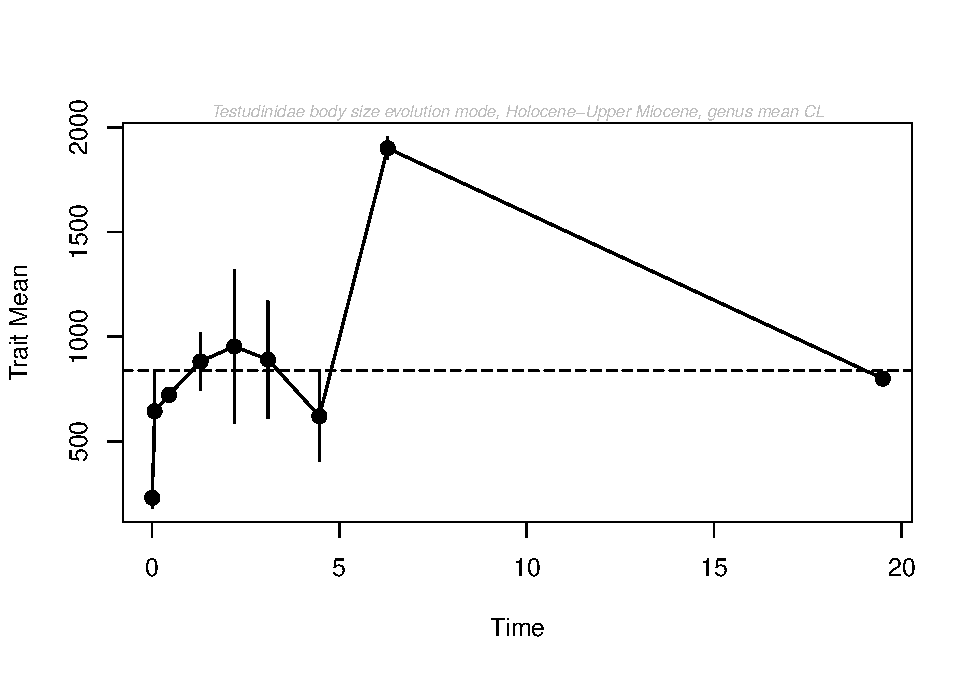
\includegraphics{MA_JJ_files/figure-latex/pTSEsI-1.pdf}
\caption{paleoTS, genera, Eurasia, insular}
\end{figure}

\begin{longtable}[]{@{}lrrrr@{}}
\caption{Model-fitting results for testudinidae, genera, Eurasia,
insular}\tabularnewline
\toprule
& logL & K & AICc & Akaike.wt\tabularnewline
\midrule
\endfirsthead
\toprule
& logL & K & AICc & Akaike.wt\tabularnewline
\midrule
\endhead
GRW & -69.56419 & 2 & 145.1284 & 0.193\tabularnewline
URW & -71.67437 & 1 & 145.9202 & 0.130\tabularnewline
Stasis & -68.31026 & 2 & 142.6205 & 0.677\tabularnewline
\bottomrule
\end{longtable}


\end{document}
